% !TeX program = pdflatex
% Single-file build for Overleaf.
% The bibliography is embedded below via filecontents; on first compile it is
% written to references.bib, then picked up by bibtex (run: pdflatex, bibtex,
% pdflatex, pdflatex). Upload the image files into an assets/ folder next to
% this main.tex (see \graphicspath).
\begin{filecontents}[overwrite]{references.bib}
% ============================================================
% Foundational Transformers
% ============================================================

@inproceedings{vaswani2017attention,
  title     = {Attention Is All You Need},
  author    = {Vaswani, Ashish and Shazeer, Noam and Parmar, Niki and Uszkoreit, Jakob and
               Jones, Llion and Gomez, Aidan N. and Kaiser, {\L}ukasz and Polosukhin, Illia},
  booktitle = {Advances in Neural Information Processing Systems},
  volume    = {30},
  year      = {2017}
}

@article{brown2020gpt3,
  title   = {Language Models are Few-Shot Learners},
  author  = {Brown, Tom and Mann, Benjamin and Ryder, Nick and Subbiah, Melanie and
             Kaplan, Jared D. and Dhariwal, Prafulla and Neelakantan, Arvind and
             Shyam, Pranav and Sastry, Girish and Askell, Amanda and others},
  journal = {Advances in Neural Information Processing Systems},
  volume  = {33},
  pages   = {1877--1901},
  year    = {2020}
}

% ============================================================
% Positional Encoding
% ============================================================

@article{su2024rope,
  title   = {{RoFormer}: Enhanced Transformer with Rotary Position Embedding},
  author  = {Su, Jianlin and Ahmed, Murtadha and Lu, Yu and Pan, Shengfeng and
             Bo, Wen and Liu, Yunfeng},
  journal = {Neurocomputing},
  volume  = {568},
  pages   = {127063},
  year    = {2024}
}

@article{peng2023yarn,
  title   = {{YaRN}: Efficient Context Window Extension of Large Language Models},
  author  = {Peng, Bowen and Quesnelle, Jeffrey and Fan, Honglu and Shippole, Enrico},
  journal = {arXiv preprint arXiv:2309.00071},
  year    = {2023}
}

@article{ding2024longrope,
  title   = {{LongRoPE}: Extending {LLM} Context Window Beyond 2 Million Tokens},
  author  = {Ding, Yiran and Zhang, Li Lyna and Zhang, Chengruidong and Xu, Yuanyuan and
             Shang, Ning and Xu, Jiahang and Yang, Fan and Yang, Mao},
  journal = {arXiv preprint arXiv:2402.13753},
  year    = {2024}
}

% ============================================================
% Triton
% ============================================================

@inproceedings{tillet2019triton,
  title     = {Triton: An Intermediate Language and Compiler for Tiled Neural Network Computations},
  author    = {Tillet, Philippe and Kung, H.~T. and Cox, David},
  booktitle = {Proceedings of the 3rd {ACM} {SIGPLAN} International Workshop on Machine Learning and Programming Languages},
  pages     = {10--19},
  year      = {2019}
}

% ============================================================
% Attention / FlashAttention
% ============================================================

@inproceedings{dao2022flashattention,
  title     = {{FlashAttention}: Fast and Memory-Efficient Exact Attention with {IO}-Awareness},
  author    = {Dao, Tri and Fu, Dan and Ermon, Stefano and Rudra, Atri and R{\'e}, Christopher},
  booktitle = {Advances in Neural Information Processing Systems},
  volume    = {35},
  pages     = {16344--16359},
  year      = {2022}
}

@inproceedings{dao2023flashattention2,
  title     = {{FlashAttention-2}: Faster Attention with Better Parallelism and Work Partitioning},
  author    = {Dao, Tri},
  booktitle = {International Conference on Learning Representations},
  year      = {2024}
}

% ============================================================
% Static sparse attention
% ============================================================

@article{child2019generating,
  title   = {Generating Long Sequences with Sparse Transformers},
  author  = {Child, Rewon and Gray, Scott and Radford, Alec and Sutskever, Ilya},
  journal = {arXiv preprint arXiv:1904.10509},
  year    = {2019}
}

% ============================================================
% Attention sinks / local window
% ============================================================

@inproceedings{xiao2023streamingllm,
  title     = {Efficient Streaming Language Models with Attention Sinks},
  author    = {Xiao, Guangxuan and Tian, Yuandong and Chen, Beidi and Han, Song and Lewis, Mike},
  booktitle = {International Conference on Learning Representations},
  year      = {2024}
}

% ============================================================
% Dynamic sparse attention (prefill)
% ============================================================

@inproceedings{jiang2024minference,
  title     = {{MI}nference 1.0: Accelerating Pre-filling for Long-Context {LLMs} via Dynamic Sparse Attention},
  author    = {Jiang, Huiqiang and Li, Yucheng and Zhang, Chengruidong and Wu, Qianhui and
               Luo, Xufang and Ahn, Surin and Han, Zhenhua and Abdi, Amir H. and
               Li, Dongsheng and Lin, Chin-Yew and Yang, Yuqing and Qiu, Lili},
  booktitle = {Advances in Neural Information Processing Systems},
  year      = {2024}
}

@inproceedings{zhang2025spargeattn,
  title     = {{SpargeAttention}: Accurate and Training-free Sparse Attention Accelerating Any Model Inference},
  author    = {Zhang, Jintao and Xiang, Chendong and Huang, Haofeng and Wei, Jia and
               Xi, Haocheng and Zhu, Jun and Chen, Jianfei},
  booktitle = {Proceedings of the 42nd International Conference on Machine Learning},
  series    = {Proceedings of Machine Learning Research},
  volume    = {267},
  publisher = {PMLR},
  year      = {2025}
}

@inproceedings{lai2025flexprefill,
  title     = {{FlexPrefill}: A Context-Aware Sparse Attention Mechanism for Efficient Long-Sequence Inference},
  author    = {Lai, Xunhao and Lu, Jianqiao and Luo, Yao and Ma, Yiyuan and Zhou, Xun},
  booktitle = {International Conference on Learning Representations},
  year      = {2025}
}

@article{xu2025xattention,
  title   = {{XAttention}: Block Sparse Attention with Antidiagonal Scoring},
  author  = {Xu, Ruyi and Xiao, Guangxuan and Huang, Haofeng and Guo, Junxian and Han, Song},
  journal = {arXiv preprint arXiv:2503.16428},
  year    = {2025}
}

% ============================================================
% K-matrix sparsity (prefill, parallel line)
% ============================================================

@article{qi2024deltallm,
  title   = {{DeltaLLM}: A Training-Free Framework Exploiting Temporal Sparsity for Efficient Edge {LLM} Inference},
  author  = {Qi, Jiawen and Gao, Chang and Ren, Zhaochun and Chen, Qinyu},
  journal = {TODO: add arXiv ID or venue},
  year    = {2024}
}

% ============================================================
% Low-rank KV compression
% ============================================================

@inproceedings{saxena2024eigenattention,
  title     = {Eigen Attention: Attention in Low-Rank Space for {KV} Cache Compression},
  author    = {Saxena, Utkarsh and Saha, Gobinda and Choudhary, Sakshi and Roy, Kaushik},
  booktitle = {Findings of the Association for Computational Linguistics: {EMNLP} 2024},
  year      = {2024}
}

@article{deepseekai2024deepseekv2,
  title   = {{DeepSeek-V2}: A Strong, Economical, and Efficient Mixture-of-Experts Language Model},
  author  = {{DeepSeek-AI}},
  journal = {arXiv preprint arXiv:2405.04434},
  year    = {2024}
}

% ============================================================
% KV cache compression (decoding)
% ============================================================

@inproceedings{zhang2023h2o,
  title     = {{H2O}: Heavy-Hitter Oracle for Efficient Generative Inference of Large Language Models},
  author    = {Zhang, Zhenyu and Sheng, Ying and Zhou, Tianyi and Chen, Tianlong and
               Zheng, Lianmin and Cai, Ruisi and Song, Zhao and Tian, Yuandong and
               R{\'e}, Christopher and Barrett, Clark and Wang, Zhangyang and Chen, Beidi},
  booktitle = {Advances in Neural Information Processing Systems},
  year      = {2023}
}

@article{li2024snapkv,
  title   = {{SnapKV}: {LLM} Knows What You are Looking for Before Generation},
  author  = {Li, Yuhong and Huang, Yingbing and Yang, Bowen and Venkitesh, Bharat and
             Locatelli, Acyr and Ye, Hanchen and Cai, Tianle and Lewis, Patrick and Chen, Deming},
  journal = {arXiv preprint arXiv:2404.14469},
  year    = {2024}
}

@article{zhang2024cam,
  title   = {{CaM}: Cache Merging for Memory-efficient {LLMs} Inference},
  author  = {Zhang, Yuxin and Du, Yuxuan and Luo, Gen and Zhong, Yunshan and
             Zhang, Zhenyu and Liu, Shiwei and Ji, Rongrong},
  journal = {TODO: add arXiv ID or venue},
  year    = {2024}
}

@article{wang2024kvmerger,
  title   = {Model Tells You Where to Merge: Adaptive {KV} Cache Merging for {LLMs} on Long-Context Tasks},
  author  = {Wang, Zheng and Jin, Boxiao and Yu, Zhongzhi and Zhang, Minjia},
  journal = {arXiv preprint arXiv:2407.08454},
  year    = {2024}
}

% ============================================================
% Long-context benchmarks
% ============================================================

@inproceedings{kuratov2024babilong,
  title     = {{BABILong}: Testing the Limits of {LLMs} with Long Context Reasoning-in-a-Haystack},
  author    = {Kuratov, Yuri and Bulatov, Aydar and Anokhin, Petr and Rodkin, Ivan and
               Sorokin, Dmitry and Sorokin, Artyom and Burtsev, Mikhail},
  booktitle = {Advances in Neural Information Processing Systems},
  year      = {2024}
}

@inproceedings{hsieh2024ruler,
  title     = {{RULER}: What's the Real Context Size of Your Long-Context Language Models?},
  author    = {Hsieh, Cheng-Ping and Sun, Simeng and Kriman, Samuel and Acharya, Shantanu and
               Rekesh, Dima and Jia, Fei and Zhang, Yang and Ginsburg, Boris},
  booktitle = {Proceedings of the First Conference on Language Modeling},
  year      = {2024}
}

@inproceedings{bai2024longbench,
  title     = {{LongBench}: A Bilingual, Multitask Benchmark for Long Context Understanding},
  author    = {Bai, Yushi and Lv, Xin and Zhang, Jiajie and Lyu, Hongchang and Tang, Jiankai and
               Huang, Zhidian and Du, Zhengxiao and Liu, Xiao and Zeng, Aohan and Hou, Lei and
               Dong, Yuxiao and Tang, Jie and Li, Juanzi},
  booktitle = {Proceedings of the 62nd Annual Meeting of the Association for Computational Linguistics},
  year      = {2024}
}

% ============================================================
% Hybrid prefill + decoding
% ============================================================

@article{xiao2024infllm,
  title   = {{InfLLM}: Training-Free Long-Context Extrapolation for {LLMs} with an Efficient Context Memory},
  author  = {Xiao, Chaojun and Zhang, Pengle and Han, Xu and Xiao, Guangxuan and
             Lin, Yankai and Zhang, Zhengyan and Liu, Zhiyuan and Sun, Maosong},
  journal = {arXiv preprint arXiv:2402.04617},
  year    = {2024}
}

% ============================================================
% Video understanding benchmark
% ============================================================

@inproceedings{fu2024videomme,
  title     = {Video-{MME}: The First-Ever Comprehensive Evaluation Benchmark of Multi-modal {LLMs} in Video Analysis},
  author    = {Fu, Chaoyou and Dai, Yuhan and Luo, Yongdong and Li, Lei and Ren, Shuhuai and
               Zhang, Renrui and Wang, Zihan and Zhou, Chenyu and Shen, Yunhang and Zhang, Mengdan and
               Chen, Peixian and Li, Yanwei and Lin, Shaohui and Zhao, Sirui and Li, Ke and Xu, Tong and
               Zheng, Xiawu and Chen, Enhong and Ji, Rongrong and Sun, Xing},
  booktitle = {Proceedings of the IEEE/CVF Conference on Computer Vision and Pattern Recognition (CVPR)},
  year      = {2025}
}
\end{filecontents}

\documentclass[11pt]{article}
\usepackage[margin=1in]{geometry}
\usepackage[numbers]{natbib}
\usepackage{amsmath}
\usepackage{graphicx}
\graphicspath{{assets/}{./}}
\usepackage{subcaption}
\usepackage{hyperref}
\usepackage{booktabs}
\usepackage{tikz}
\usetikzlibrary{arrows.meta}
\usepackage{pgfplots}
\pgfplotsset{compat=1.18}

% Encourage floats to sit near their reference instead of drifting to the end
\renewcommand{\topfraction}{0.9}
\renewcommand{\bottomfraction}{0.8}
\renewcommand{\textfraction}{0.07}
\renewcommand{\floatpagefraction}{0.75}
\setcounter{topnumber}{3}
\setcounter{bottomnumber}{2}
\setcounter{totalnumber}{5}

\title{DeltaAttention}
\author{}
\date{}

\begin{document}
\maketitle

% ==================== abstract ====================
\begin{abstract}
Long-context prefill is dominated by the cost of attention, which grows quadratically with sequence length. Most training-free work speeds this up by exploiting the sparsity of the attention matrix. We start from a different observation: adjacent query and key vectors are highly similar at the token level, so the $Q$ and $K$ matrices can be compressed along the sequence dimension.

We apply this single idea in three ways. Delta-KV applies it as a standalone optimization, packing the key and value matrices along the sequence dimension to halve the attention operations while keeping accuracy competitive and reaching up to a 2$\times$ prefill speedup. DeltaXAttention applies the same packing inside the tiles that XAttention selects. Delta-based tile scoring (DPXA) uses the delta representation to estimate tile importance cheaply for block-sparse attention.

DPXA is the strongest of the three. On LLaMA-3.1 8B Instruct it is essentially lossless on RULER and competitive on LongBench, it holds up on Qwen2.5-7B, and it transfers to long video understanding on Qwen2-VL. On Llama it produces a higher-quality tile-importance signal than XAttention at a fraction of the scoring cost, and across both models it matches or beats XAttention's speedup at every setting we test. Its one weakness is a drop on the Qwen aggregation tasks, which does not carry over to the real-world LongBench benchmark. Overall this places DPXA in a competitive position among training-free sparse attention methods.

These results show that adjacency redundancy in $Q$ and $K$ is a useful and largely unexplored area for accelerating long-context attention.
\end{abstract}
\newpage

\setcounter{tocdepth}{2}
\tableofcontents
\newpage

% ==================== introduction ====================
\section{Introduction}

Before the Transformer era, language models were built on recurrent neural networks (RNNs) and their variants such as LSTMs and GRUs.
These models were used in small-scale conversational assistants like Siri and Alexa, but their usefulness was limited.
RNNs encode context into a fixed-size hidden state, which means they forget information as sequences grow longer and the hidden state gets diluted.
More importantly, they process text sequentially token by token, making it impossible to parallelize training across the sequence.
This sequential bottleneck kept these models small.

The groundbreaking paper \textit{Attention Is All You Need}~\citep{vaswani2017attention} changed the field.
Transformers process all tokens in a sequence simultaneously, making it possible to train on massive datasets using GPU parallelism.
Scaled to billions of parameters on web data, GPT-3~\citep{brown2020gpt3} could do in-context learning, translation, coding, and reasoning without any task-specific training.
The scale of the data and model allowed a certain amount of generalization that earlier architectures could not achieve.

The mechanism behind this is the attention module.
Each token attends to every other token in the sequence simultaneously, allowing the model to capture long-range dependencies. However, computing attention for a sequence of length $n$ requires $O(n^2)$ time and memory, since every token pair must be considered. This quadratic scaling kept context windows short.
GPT-3, for instance, was limited to 2048 tokens.

FlashAttention~\citep{dao2022flashattention} addressed the memory side of this by computing attention in tiles in on-chip SRAM rather than materializing the full attention matrix in HBM, bringing memory use down to linear.
On handling token position, the original Transformer used absolute positional encodings: positions were essentially hardcoded, so models simply broke on sequences longer than they were trained on. RoPE~\citep{su2024rope} encodes position relative to other tokens rather than absolutely, which generalizes much better to longer sequences, and extensions such as YaRN~\citep{peng2023yarn} and LongRoPE~\citep{ding2024longrope} pushed this further. Together, these advances enabled the jump to context windows of 100k tokens and beyond.

Long context allowed a world of practical applications for LLMs. Coding agents can now take in entire codebases and reason about them. Long documents such as legal contracts, research papers, and financial reports can be analyzed in a single pass. Retrieval-Augmented Generation (RAG) feeds retrieved documents directly into the model context, allowing LLMs to answer questions grounded in external knowledge that was not part of their training data. These applications share a common bottleneck.
LLM inference consists of two stages: the prefill stage, which processes the entire input prompt in a single forward pass, and the decoding stage, which generates output tokens one by one.
As context length grows, the quadratic time complexity of attention makes prefill increasingly expensive.
Memory was the original wall; FlashAttention removed it but did not address the time complexity: computing attention on long contexts is slow.

A large body of work aims to accelerate attention for long context tasks by exploiting the empirical sparsity of the attention matrix: most tokens only attend strongly to a small local window and a few distant positions, so many token pair interactions do not need to be computed at all.
Early work used fixed sparse patterns~\citep{child2019generating}; more recent methods determine the pattern dynamically based on the input~\citep{jiang2024minference, lai2025flexprefill, xu2025xattention}.

This thesis exploits the insight that adjacent tokens have similar key vectors, with high cosine similarity between neighboring keys. This redundancy in $K$ is already documented in prior work~\citep{wang2024kvmerger, qi2024deltallm}. We show that the same holds for query vectors: adjacent queries are also highly similar. Unlike the sparsity of the attention matrix, this adjacency redundancy lives in the $Q$ and $K$ matrices before attention is computed, so it can be exploited independently of existing sparse attention methods or layered on top of them.

We apply this single insight to three prefill acceleration applications:
\begin{itemize}
    \item \textbf{Delta-KV compression.} We compress the key and value matrices along the sequence dimension before the $QK$ multiplication, reducing attention FLOPs proportionally to the compression ratio. We provide custom Triton kernels that turn this into wall-clock speedup, not just a theoretical reduction in FLOPs (Sections~\ref{sec:preprocessing}--\ref{sec:flash_attention_adaptation}).
    \item \textbf{DeltaXAttention.} We apply the same compression on top of a block-sparse method, XAttention, compressing the keys inside the tiles it already selects to accelerate it further (Section~\ref{sec:xattention_adaptation}).
    \item \textbf{Delta-based tile scoring (DPXA).} We use the adjacency structure as a tile importance estimator for block-sparse attention, choosing which tiles to compute while sampling far less of each tile than existing estimators (Section~\ref{sec:delta_tile_scoring}).
\end{itemize}

These three are not equal contributions. The first two demonstrate what delta compression can and cannot do as a prefill optimization, and both turn out to have limited practical value: Delta-KV compression is dominated by existing methods as a standalone optimization, and DeltaXAttention saves KV loads that XAttention can already match by skipping tiles. DPXA is where the idea fits naturally. It is the strongest of the three, matching full attention on RULER for Llama, where it produces a higher-quality tile-importance signal than XAttention at a fraction of the scoring cost, and matching or beating XAttention's speedup across both models.

% ==================== preliminary ====================
\section{Preliminaries}

\subsection{Transformer Overview}

\begin{figure}[!ht]
    \centering
    
\includegraphics[width=\textwidth]{assets/transformer_overview.jpeg}
    \caption{Overview of a Transformer language model}
    \label{fig:transformer_overview}
\end{figure}

A Transformer language model processes text as follows (Figure~\ref{fig:transformer_overview}).
Text is first split into tokens, and each token is mapped to a vector by looking it up in a learned embedding table.
This gives a sequence of vectors of shape $n \times d$, where $n$ is the sequence length and $d$ is the embedding dimension.

These vectors are then passed through a chain of $N$ identical layers.
Each layer consists of two modules: an attention module followed by an MLP, each with a residual connection.
Through these layers, the embedding of each token is updated to incorporate information from the rest of the sequence.

After the final layer, the embedding of the last token is projected back to the vocabulary size by an unembedding matrix, producing a logit for each vocabulary entry.
A softmax turns these logits into a probability distribution, and the next token is sampled from it.
This token is appended to the sequence, and the whole forward pass is run again to generate the token after that.
Generation continues until an end-of-sequence token is produced.

\subsection{Attention Block}

This section explains the inner workings of the attention block shown in Figure~\ref{fig:transformer_overview}.



\subsubsection{Self-Attention}
\label{sec:self_attention}

\begin{figure}[!ht]
    \centering
    
\includegraphics[width=0.75\textwidth]{assets/Self_Attention.png}
    \caption{Self-attention mechanism.}
    \label{fig:self_attention}
\end{figure}

Self-attention is the operation inside each attention block (Figure~\ref{fig:self_attention}).
The input hidden state matrix of shape $n \times d$ is projected to three matrices, queries $Q$, keys $K$, and values $V$, each of shape $n \times l$, using learned projection matrices.

The attention scores are computed as:
\begin{equation}
    \text{Attention}(Q, K, V) = \text{softmax}\!\left(\frac{QK^\top}{\sqrt{l}}\right) V
\end{equation}

The $QK^\top$ product gives an $n \times n$ scores matrix where entry $(a, b)$ is the dot product of token $a$'s query vector with token $b$'s key vector.
Intuitively, the query of a token encodes what it is looking for, and the key of a token encodes what it has to offer.
Their dot product measures how relevant token $b$ is to token $a$.
Dividing by $\sqrt{l}$ keeps the dot products from growing too large before the softmax.

Applying softmax row-wise turns each row into a probability distribution, the attention weights, which say how much each token attends to every other token.

The attention weights are then multiplied with the value matrix $V$ to produce the attention output: each token's output is a weighted sum of all value vectors, where the weights come from its row of the attention matrix.
Intuitively, the value vector of a token encodes the information it contributes to other tokens, and the attention weight determines how much of that contribution is applied. As shown in Figure~\ref{fig:transformer_overview}, this attention output is then added back to the input hidden state via a residual connection.

\subsubsection{Multi-Head Attention}

\begin{figure}[!ht]
    \centering
    
\includegraphics[width=0.7\textwidth]{assets/mha.jpeg}
    \caption{Multi-head attention.}
    \label{fig:mha}
\end{figure}

The attention module inside each Transformer layer is a multi-head attention (MHA) block (Figure~\ref{fig:mha}).
Rather than running a single attention computation over the full embedding dimension, MHA runs $h$ attention computations (heads) in parallel, each operating in a smaller subspace of width $l = d / h$.
The input to the block is the hidden state matrix of shape $n \times d$, where $n$ is the sequence length and $d$ is the embedding dimension.
Each head has its own learned projection matrices that map the full $d$-dimensional input down to $l$ dimensions, producing per-head queries, keys, and values of shape $n \times l$.
Each head sees the full sequence and the full embedding, but through its own projection, different heads facilitate different attention patterns and capture different types of token interactions.
The output of each head has the same shape $n \times l$, and the $h$ outputs are concatenated along the embedding dimension to give a final output of shape $n \times d$, matching the input.


\subsection{FlashAttention}

Materializing the full $n \times n$ attention scores matrix has two critical problems.

The first is memory capacity. The matrix grows quadratically with sequence length: at 10k tokens it is roughly 200 MB per head, at 100k tokens it is around 20 GB per head, and at 1 million tokens it exceeds 2 TB per head. MHA runs $h$ heads in parallel, so these numbers scale by $h$; a model like LLaMA-3.1 8B uses 32 heads. An H100 has 80 GB of HBM, so at long sequences the scores matrices alone exhaust GPU memory by a large factor.

The second problem is memory bandwidth. Even when the matrix fits, standard attention is bottlenecked by repeated data movement between HBM and the small on-chip SRAM. Computing attention requires multiple passes over the scores: write scores to HBM, read them back for softmax, write the result, read it again for the matmul with $V$. Each of these round trips is slow, and they dominate the runtime at long sequences.

FlashAttention~\cite{dao2022flashattention} solves both problems by computing attention in tiles that fit in SRAM. Within each tile, the score computation, softmax, and matmul with $V$ are fused into a single pass, so intermediate results are never written to HBM. This requires an incremental softmax update to accumulate the correct result across tiles without materializing the full scores matrix. The peak memory footprint drops from $O(n^2)$ to $O(n)$, and the intermediate HBM read/writes are eliminated.

\subsubsection{FlashAttention Algorithm}
\label{sec:flashattention_algorithm}

$Q$, $K$, and $V$ are divided into fixed-size blocks along the sequence dimension (typically 64 or 128 tokens per block). The outer loop iterates over $Q$ blocks; for each $Q$ block, an inner loop iterates over all $K$ and $V$ blocks in sequence.

For each ($Q$ block, $K$/$V$ block) pair, three steps happen in SRAM:

\begin{itemize}
    \item The $Q$ block and $K$ block are multiplied to produce an attention scores tile of shape $B_q \times B_k$, where $B_q$ is the query block size and $B_k$ is the key block size.
    \item Online softmax is applied to the scores tile. Standard softmax requires the full row to normalize, but online softmax maintains a running maximum and a running sum that are corrected as each new tile arrives, producing numerically identical results without having the full row in memory.
    \item The attention weights tile is multiplied with the $V$ block to get a partial attention output of shape $B_q \times d$. This is added to a running output accumulator for the current $Q$ block, which collects the contributions from all $K$/$V$ blocks seen so far.
\end{itemize}

Once all $K$/$V$ blocks have been processed, the running accumulator holds the sum of all partial contributions. It is rescaled by the final softmax normalizer from the online softmax and written back to HBM as the attention output for this $Q$ block.

FlashAttention-1 parallelizes this computation over the batch and head dimensions. FlashAttention-2~\cite{dao2023flashattention2} additionally parallelizes over $Q$ blocks: each kernel instance handles one $Q$ block independently, iterating over all $K$ and $V$ blocks on its own. Since there are no dependencies between $Q$ blocks, this is feasible and enables significantly more parallelism.

\subsubsection{FlashAttention Demonstration}

Figure~\ref{fig:flashattn_snapshot} shows a FlashAttention~2 program computing the second query block ($Q_2$), with block size~2, sequence length~8, and head dimension~1. Other programs handle the remaining $Q$ blocks in parallel. The gray upper-triangular blocks of $S$ mark KV blocks skipped entirely: every token in those blocks lies in the future of the corresponding query block.

In iteration~1 (left), $Q_2$ and $K_1$ are loaded into SRAM and multiplied to produce scores tile $S_{21}$. After online softmax, $S_{21}$ is multiplied with $V_1$ and accumulated into $O_2$.

In iteration~2 (right), the $K$ and $V$ blocks advance to block~2. $Q_2$ and $K_2$ produce tile $S_{22}$, which is multiplied with $V_2$ and again accumulated into $O_2$. The program stops here: blocks $K_3$ and beyond lie entirely in the future relative to $Q_2$, so they are skipped due to causality.

After all $K$/$V$ blocks have been processed, $O_2$ holds the correct attention output for the tokens in $Q_2$, rescaled by the final softmax normalizer.

%% ---- begin diagrams/flash_attention_demonstration ----
\begin{figure}[h]
\centering
\resizebox{\textwidth}{!}{
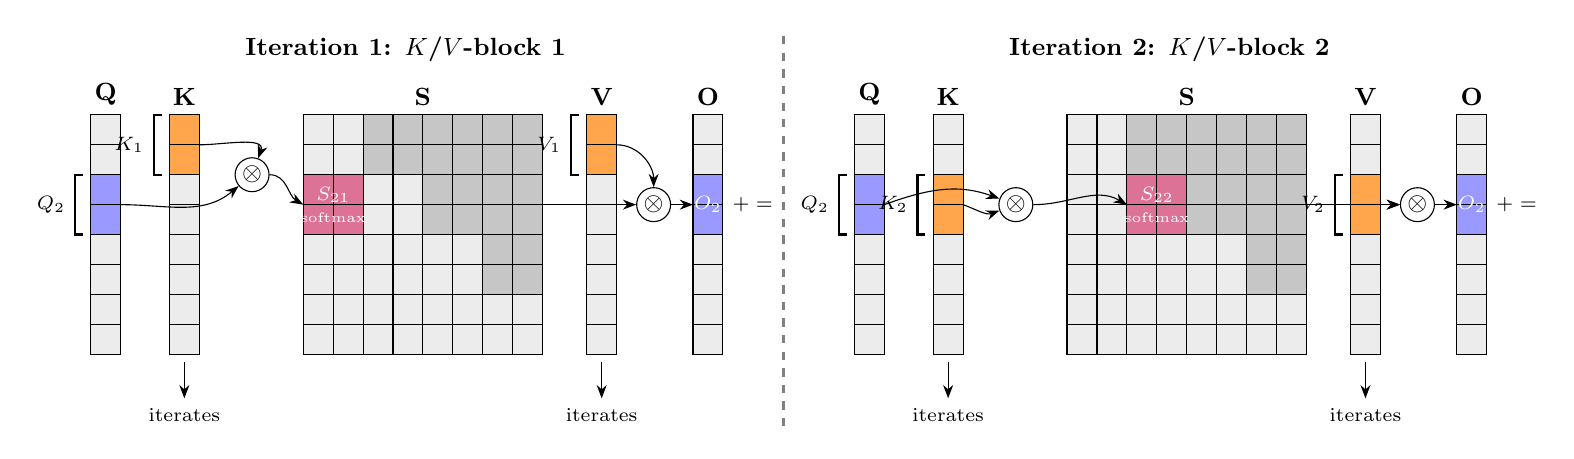
\begin{tikzpicture}
  % cell=0.38cm; Q,K,V,O: 8x1; S: 8x8
  % Iter 1: Q=0, K=1.0, qkmul=2.05, S=2.7, V=6.3, smul=7.15, O=7.65
  % Iter 2: same + xoff=9.7
  \colorlet{bblue}{blue!40}
  \colorlet{borange}{orange!70}
  \colorlet{bpurple}{purple!55}
  \colorlet{bgray}{gray!15}
  \colorlet{bmask}{gray!45}

  %%% ITERATION 1 %%%

  % Q (8x1), x=0; Q2=rows 2-3
  \foreach \r in {0,...,7} {
    \fill[bgray] (0,{-\r*0.38}) rectangle (0.38,{-\r*0.38-0.38});
    \draw        (0,{-\r*0.38}) rectangle (0.38,{-\r*0.38-0.38});
  }
  \foreach \r in {2,3} {
    \fill[bblue] (0,{-\r*0.38}) rectangle (0.38,{-\r*0.38-0.38});
    \draw        (0,{-\r*0.38}) rectangle (0.38,{-\r*0.38-0.38});
  }
  \node[above,font=\small\bfseries] at (0.19,0) {Q};
  \draw[thick] (-0.10,-0.76)--(-0.20,-0.76)--(-0.20,-1.52)--(-0.10,-1.52);
  \node[left,font=\scriptsize] at (-0.20,-1.14) {$Q_2$};

  % K (8x1), x=1.0; K1=rows 0-1
  \foreach \r in {0,...,7} {
    \fill[bgray]   (1.0,{-\r*0.38}) rectangle (1.38,{-\r*0.38-0.38});
    \draw          (1.0,{-\r*0.38}) rectangle (1.38,{-\r*0.38-0.38});
  }
  \foreach \r in {0,1} {
    \fill[borange] (1.0,{-\r*0.38}) rectangle (1.38,{-\r*0.38-0.38});
    \draw          (1.0,{-\r*0.38}) rectangle (1.38,{-\r*0.38-0.38});
  }
  \node[above,font=\small\bfseries] at (1.19,0) {K};
  \draw[thick] (0.90,0)--(0.80,0)--(0.80,-0.76)--(0.90,-0.76);
  \node[left,font=\scriptsize] at (0.80,-0.38) {$K_1$};
  \draw[-{Stealth}] (1.19,-3.14)--(1.19,-3.60);
  \node[below,font=\scriptsize] at (1.19,-3.60) {iterates};

  \node[draw,circle,inner sep=1pt,font=\small] (qkmul) at (2.05,-0.76) {$\otimes$};

  % S (8x8), x=2.7; S21=rows 2-3, cols 0-1
  \foreach \r in {0,...,7} { \foreach \c in {0,...,7} {
    \fill[bgray] ({2.7+\c*0.38},{-\r*0.38}) rectangle ({2.7+\c*0.38+0.38},{-\r*0.38-0.38});
    \draw        ({2.7+\c*0.38},{-\r*0.38}) rectangle ({2.7+\c*0.38+0.38},{-\r*0.38-0.38});
  }}
  % causal mask: upper-triangular blocks (block-col > block-row), block size 2
  \foreach \br in {0,...,3} { \foreach \bc in {0,...,3} {
    \pgfmathparse{int(\bc>\br)}
    \ifnum\pgfmathresult=1
      \foreach \ri in {0,1} { \foreach \ci in {0,1} {
        \pgfmathtruncatemacro\rr{\br*2+\ri}
        \pgfmathtruncatemacro\cc{\bc*2+\ci}
        \fill[bmask] ({2.7+\cc*0.38},{-\rr*0.38}) rectangle ({2.7+\cc*0.38+0.38},{-\rr*0.38-0.38});
        \draw        ({2.7+\cc*0.38},{-\rr*0.38}) rectangle ({2.7+\cc*0.38+0.38},{-\rr*0.38-0.38});
      }}
    \fi
  }}
  \foreach \r in {2,3} { \foreach \c in {0,1} {
    \fill[bpurple] ({2.7+\c*0.38},{-\r*0.38}) rectangle ({2.7+\c*0.38+0.38},{-\r*0.38-0.38});
    \draw          ({2.7+\c*0.38},{-\r*0.38}) rectangle ({2.7+\c*0.38+0.38},{-\r*0.38-0.38});
  }}
  \node[above,font=\small\bfseries] at (4.22,0) {S};
  \node[white,font=\scriptsize,align=center] at (3.08,-1.14) {$S_{21}$\\\tiny softmax};

  % V (8x1), x=6.3; V1=rows 0-1
  \foreach \r in {0,...,7} {
    \fill[bgray]   (6.3,{-\r*0.38}) rectangle (6.68,{-\r*0.38-0.38});
    \draw          (6.3,{-\r*0.38}) rectangle (6.68,{-\r*0.38-0.38});
  }
  \foreach \r in {0,1} {
    \fill[borange] (6.3,{-\r*0.38}) rectangle (6.68,{-\r*0.38-0.38});
    \draw          (6.3,{-\r*0.38}) rectangle (6.68,{-\r*0.38-0.38});
  }
  \node[above,font=\small\bfseries] at (6.49,0) {V};
  \draw[thick] (6.20,0)--(6.10,0)--(6.10,-0.76)--(6.20,-0.76);
  \node[left,font=\scriptsize] at (6.10,-0.38) {$V_1$};
  \draw[-{Stealth}] (6.49,-3.14)--(6.49,-3.60);
  \node[below,font=\scriptsize] at (6.49,-3.60) {iterates};

  \node[draw,circle,inner sep=1pt,font=\small] (smul) at (7.15,-1.14) {$\otimes$};

  % O (8x1), x=7.65; O2=rows 2-3
  \foreach \r in {0,...,7} {
    \fill[bgray]  (7.65,{-\r*0.38}) rectangle (8.03,{-\r*0.38-0.38});
    \draw         (7.65,{-\r*0.38}) rectangle (8.03,{-\r*0.38-0.38});
  }
  \foreach \r in {2,3} {
    \fill[bblue]  (7.65,{-\r*0.38}) rectangle (8.03,{-\r*0.38-0.38});
    \draw         (7.65,{-\r*0.38}) rectangle (8.03,{-\r*0.38-0.38});
  }
  \node[above,font=\small\bfseries] at (7.84,0) {O};
  \node[white,font=\scriptsize] at (7.84,-1.14) {$O_2$};
  \node[right,font=\scriptsize] at (8.03,-1.14) {$+=$};

  % Arrows iter 1
  \draw[-{Stealth}] (0.38,-1.14) to[out=0,in=220] (qkmul);
  \draw[-{Stealth}] (1.38,-0.38) to[out=0,in=70]  (qkmul);
  \draw[-{Stealth}] (qkmul) to[out=0,in=150] (2.7,-1.14);
  \draw[-{Stealth}] (3.46,-1.14)--(smul);
  \draw[-{Stealth}] (6.68,-0.38) to[out=0,in=90] (smul);
  \draw[-{Stealth}] (smul)--(7.65,-1.14);

  \node[above,font=\small\bfseries] at (4.0,0.55) {Iteration 1: $K$/$V$-block 1};

  %%% SEPARATOR %%%
  \draw[dashed, thick, gray] (8.8, 1.0) -- (8.8, -4.0);

  %%% ITERATION 2 (xoff=9.7) %%%

  % Q (8x1), x=9.7; Q2=rows 2-3
  \foreach \r in {0,...,7} {
    \fill[bgray] (9.7,{-\r*0.38}) rectangle (10.08,{-\r*0.38-0.38});
    \draw        (9.7,{-\r*0.38}) rectangle (10.08,{-\r*0.38-0.38});
  }
  \foreach \r in {2,3} {
    \fill[bblue] (9.7,{-\r*0.38}) rectangle (10.08,{-\r*0.38-0.38});
    \draw        (9.7,{-\r*0.38}) rectangle (10.08,{-\r*0.38-0.38});
  }
  \node[above,font=\small\bfseries] at (9.89,0) {Q};
  \draw[thick] (9.60,-0.76)--(9.50,-0.76)--(9.50,-1.52)--(9.60,-1.52);
  \node[left,font=\scriptsize] at (9.50,-1.14) {$Q_2$};

  % K (8x1), x=10.7; K2=rows 2-3
  \foreach \r in {0,...,7} {
    \fill[bgray]   (10.7,{-\r*0.38}) rectangle (11.08,{-\r*0.38-0.38});
    \draw          (10.7,{-\r*0.38}) rectangle (11.08,{-\r*0.38-0.38});
  }
  \foreach \r in {2,3} {
    \fill[borange] (10.7,{-\r*0.38}) rectangle (11.08,{-\r*0.38-0.38});
    \draw          (10.7,{-\r*0.38}) rectangle (11.08,{-\r*0.38-0.38});
  }
  \node[above,font=\small\bfseries] at (10.89,0) {K};
  \draw[thick] (10.60,-0.76)--(10.50,-0.76)--(10.50,-1.52)--(10.60,-1.52);
  \node[left,font=\scriptsize] at (10.50,-1.14) {$K_2$};
  \draw[-{Stealth}] (10.89,-3.14)--(10.89,-3.60);
  \node[below,font=\scriptsize] at (10.89,-3.60) {iterates};

  \node[draw,circle,inner sep=1pt,font=\small] (qkmulB) at (11.75,-1.14) {$\otimes$};

  % S (8x8), x=12.4; S22=rows 2-3, cols 2-3
  \foreach \r in {0,...,7} { \foreach \c in {0,...,7} {
    \fill[bgray] ({12.4+\c*0.38},{-\r*0.38}) rectangle ({12.4+\c*0.38+0.38},{-\r*0.38-0.38});
    \draw        ({12.4+\c*0.38},{-\r*0.38}) rectangle ({12.4+\c*0.38+0.38},{-\r*0.38-0.38});
  }}
  % causal mask: upper-triangular blocks (block-col > block-row), block size 2
  \foreach \br in {0,...,3} { \foreach \bc in {0,...,3} {
    \pgfmathparse{int(\bc>\br)}
    \ifnum\pgfmathresult=1
      \foreach \ri in {0,1} { \foreach \ci in {0,1} {
        \pgfmathtruncatemacro\rr{\br*2+\ri}
        \pgfmathtruncatemacro\cc{\bc*2+\ci}
        \fill[bmask] ({12.4+\cc*0.38},{-\rr*0.38}) rectangle ({12.4+\cc*0.38+0.38},{-\rr*0.38-0.38});
        \draw        ({12.4+\cc*0.38},{-\rr*0.38}) rectangle ({12.4+\cc*0.38+0.38},{-\rr*0.38-0.38});
      }}
    \fi
  }}
  % active tile: S22 is a diagonal block (bc==br==1), so all 4 cells are processed
  \foreach \r in {2,3} { \foreach \c in {2,3} {
    \fill[bpurple] ({12.4+\c*0.38},{-\r*0.38}) rectangle ({12.4+\c*0.38+0.38},{-\r*0.38-0.38});
    \draw          ({12.4+\c*0.38},{-\r*0.38}) rectangle ({12.4+\c*0.38+0.38},{-\r*0.38-0.38});
  }}
  \node[above,font=\small\bfseries] at (13.92,0) {S};
  \node[white,font=\scriptsize,align=center] at (13.54,-1.14) {$S_{22}$\\\tiny softmax};

  % V (8x1), x=16.0; V2=rows 2-3
  \foreach \r in {0,...,7} {
    \fill[bgray]   (16.0,{-\r*0.38}) rectangle (16.38,{-\r*0.38-0.38});
    \draw          (16.0,{-\r*0.38}) rectangle (16.38,{-\r*0.38-0.38});
  }
  \foreach \r in {2,3} {
    \fill[borange] (16.0,{-\r*0.38}) rectangle (16.38,{-\r*0.38-0.38});
    \draw          (16.0,{-\r*0.38}) rectangle (16.38,{-\r*0.38-0.38});
  }
  \node[above,font=\small\bfseries] at (16.19,0) {V};
  \draw[thick] (15.90,-0.76)--(15.80,-0.76)--(15.80,-1.52)--(15.90,-1.52);
  \node[left,font=\scriptsize] at (15.80,-1.14) {$V_2$};
  \draw[-{Stealth}] (16.19,-3.14)--(16.19,-3.60);
  \node[below,font=\scriptsize] at (16.19,-3.60) {iterates};

  \node[draw,circle,inner sep=1pt,font=\small] (smulB) at (16.85,-1.14) {$\otimes$};

  % O (8x1), x=17.35; O2=rows 2-3
  \foreach \r in {0,...,7} {
    \fill[bgray]  (17.35,{-\r*0.38}) rectangle (17.73,{-\r*0.38-0.38});
    \draw         (17.35,{-\r*0.38}) rectangle (17.73,{-\r*0.38-0.38});
  }
  \foreach \r in {2,3} {
    \fill[bblue]  (17.35,{-\r*0.38}) rectangle (17.73,{-\r*0.38-0.38});
    \draw         (17.35,{-\r*0.38}) rectangle (17.73,{-\r*0.38-0.38});
  }
  \node[above,font=\small\bfseries] at (17.54,0) {O};
  \node[white,font=\scriptsize] at (17.54,-1.14) {$O_2$};
  \node[right,font=\scriptsize] at (17.73,-1.14) {$+=$};

  % Arrows iter 2
  \draw[-{Stealth}] (10.08,-1.14) to[out=20,in=160]  (qkmulB);
  \draw[-{Stealth}] (11.08,-1.14) to[out=-20,in=200] (qkmulB);
  \draw[-{Stealth}] (qkmulB) to[out=0,in=150] (13.16,-1.14);
  \draw[-{Stealth}] (13.92,-1.14)--(smulB);
  \draw[-{Stealth}] (16.38,-1.14)--(smulB);
  \draw[-{Stealth}] (smulB)--(17.35,-1.14);

  \node[above,font=\small\bfseries] at (13.7,0.55) {Iteration 2: $K$/$V$-block 2};

\end{tikzpicture}
}
\caption{Two consecutive inner-loop iterations for $Q$-block 2.}
\label{fig:flashattn_snapshot}
\end{figure}
%% ---- end diagrams/flash_attention_demonstration ----

\subsection{Local Attention Window}
\label{sec:local_attention_window}

Attention in LLMs is empirically sparse: tokens strongly attend to their neighbors and a few distant tokens. \citet{xiao2023streamingllm} identified two regions that receive strong attention. The first is a narrow band along the diagonal, the \textbf{critical diagonal}, meaning tokens attend mostly to their neighbors. The second is the first few tokens of the sequence, the attention sink.

Figure~\ref{fig:exact_window} shows this across an early, middle, and late layer of Qwen1.5-0.5B. Every layer shows the same structure: high attention weights on the diagonal, and a vertical band on the first tokens (the attention sink) that grows stronger in the deeper layers.

\begin{figure}[!ht]
    \centering
    \setlength{\fboxsep}{3pt}%
    \setlength{\fboxrule}{0.4pt}%
    \begin{subfigure}[b]{0.30\textwidth}
        \centering
        \fbox{
\includegraphics[width=\linewidth]{assets/attn_window_early}}
        \caption{Early layer}
    \end{subfigure}
    \hspace{0.02\textwidth}%
    \begin{subfigure}[b]{0.30\textwidth}
        \centering
        \fbox{
\includegraphics[width=\linewidth]{assets/attn_window_mid}}
        \caption{Middle layer}
    \end{subfigure}
    \hspace{0.02\textwidth}%
    \begin{subfigure}[b]{0.30\textwidth}
        \centering
        \fbox{
\includegraphics[width=\linewidth]{assets/attn_window_late}}
        \caption{Late layer}
    \end{subfigure}
    \caption{Attention score heatmaps for one head in an early, middle, and late layer of Qwen1.5-0.5B during prefill on a 512-token sequence. Darker means higher attention. Every layer has a strong band along the critical diagonal, where each token attends to its neighbors.}
    \label{fig:exact_window}
\end{figure}

This observation motivates computing the attention exactly for tokens in the critical diagonal in prefill acceleration methods. \citet{jiang2024minference} have their A-shape attention pattern. \citet{qi2024deltallm} compute the attention value in the diagonal band exactly while compressing the rest via delta key vectors. Delta-KV and DeltaXAttention follow the same principle: the critical diagonal is processed with the full uncompressed keys and values.

\subsection{XAttention}
\label{sec:xattention}

%% ---- begin diagrams/xattention_3part ----
\begin{figure}[ht]
\centering
\resizebox{\textwidth}{!}{
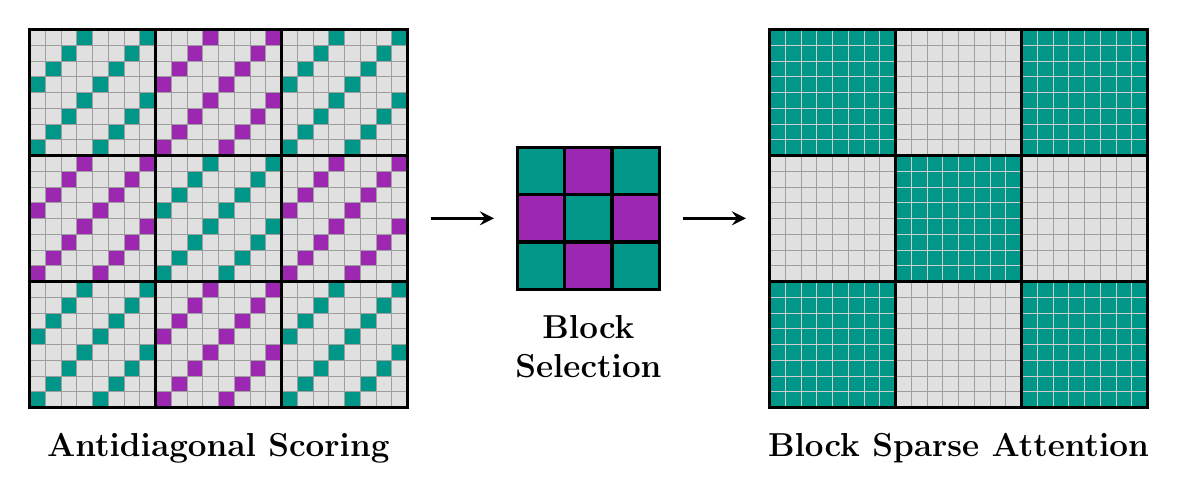
\begin{tikzpicture}[>=stealth, thick]

  % Colors
  \definecolor{selcolor}{HTML}{009688} % Teal
  \definecolor{unselcolor}{HTML}{9C27B0} % Purple
  \definecolor{bglight}{HTML}{E0E0E0}
  \definecolor{gridcolor}{HTML}{9E9E9E}

  \def\cell{0.2} % cell size for left and right
  \def\bcell{1.6} % big cell size = 8 * 0.2

  % PART 1: Antidiagonal Scoring
  \begin{scope}[shift={(0,0)}]
    % Draw background and small grid
    \fill[bglight] (0,0) rectangle (3*\bcell, -3*\bcell);
    \draw[gridcolor, very thin, step=\cell] (0,0) grid (3*\bcell, -3*\bcell);
    
    % Draw antidiagonals
    \foreach \br in {0,1,2} {
      \foreach \bc in {0,1,2} {
        % Determine if block is selected: X pattern => br == bc or br+bc == 2
        \pgfmathtruncatemacro{\issel}{(\br==\bc) || (\br+\bc==2)}
        \ifnum\issel=1
          \colorlet{dcolor}{selcolor}
        \else
          \colorlet{dcolor}{unselcolor}
        \fi
        
        \foreach \r in {0,...,7} {
          \foreach \c in {0,...,7} {
            % Antidiagonal of each S x S sub-block (S=4): the cells where
            % the local row and column index sum to S-1, i.e. r+c == 3 (mod 4).
            % Drawn over the full block without the causal mask for clarity.
            \pgfmathtruncatemacro{\isdiag}{mod(\r+\c,4)==3}
            \ifnum\isdiag=1
              \fill[dcolor] ({\bc*\bcell + \c*\cell}, {-\br*\bcell - \r*\cell}) rectangle ++(\cell, -\cell);
              \draw[gridcolor, very thin] ({\bc*\bcell + \c*\cell}, {-\br*\bcell - \r*\cell}) rectangle ++(\cell, -\cell);
            \fi
          }
        }
      }
    }
    % Draw thick big block borders
    \draw[very thick, step=\bcell] (0,0) grid (3*\bcell, -3*\bcell);
    \draw[very thick] (0,0) rectangle (3*\bcell, -3*\bcell);
    \node[below, font=\large\bfseries] at (1.5*\bcell, -3*\bcell - 0.2) {Antidiagonal Scoring};
  \end{scope}

  % Arrow 1
  \draw[->, very thick] (3*\bcell + 0.3, -1.5*\bcell) -- ++(0.8, 0);

  % PART 2: Block Selection
  % The middle grid is 3x3, let's make it smaller, e.g. cell size 0.6
  \def\mcell{0.6}
  \begin{scope}[shift={(3*\bcell + 1.4, -1.5*\bcell + 1.5*\mcell)}]
    \foreach \br in {0,1,2} {
      \foreach \bc in {0,1,2} {
        \pgfmathtruncatemacro{\issel}{(\br==\bc) || (\br+\bc==2)}
        \ifnum\issel=1
          \fill[selcolor] (\bc*\mcell, -\br*\mcell) rectangle ++(\mcell, -\mcell);
        \else
          \fill[unselcolor] (\bc*\mcell, -\br*\mcell) rectangle ++(\mcell, -\mcell);
        \fi
        \draw[very thick] (\bc*\mcell, -\br*\mcell) rectangle ++(\mcell, -\mcell);
      }
    }
    \draw[very thick] (0,0) rectangle (3*\mcell, -3*\mcell);
    \node[below, align=center, font=\large\bfseries] at (1.5*\mcell, -3*\mcell - 0.2) {Block\\Selection};
  \end{scope}

  % Arrow 2
  \draw[->, very thick] (3*\bcell + 1.4 + 3*\mcell + 0.3, -1.5*\bcell) -- ++(0.8, 0);

  % PART 3: Block Sparse Attention
  \begin{scope}[shift={(3*\bcell + 1.4 + 3*\mcell + 1.4, 0)}]
    \fill[bglight] (0,0) rectangle (3*\bcell, -3*\bcell);
    \draw[gridcolor, very thin, step=\cell] (0,0) grid (3*\bcell, -3*\bcell);
    
    \foreach \br in {0,1,2} {
      \foreach \bc in {0,1,2} {
        \pgfmathtruncatemacro{\issel}{(\br==\bc) || (\br+\bc==2)}
        \ifnum\issel=1
          \fill[selcolor] (\bc*\bcell, -\br*\bcell) rectangle ++(\bcell, -\bcell);
          % We can re-draw the small grid over it if we want it to look like the original
          \draw[gridcolor!50!white, very thin, step=\cell, shift={(\bc*\bcell, -\br*\bcell)}] (0,0) grid (\bcell, -\bcell);
        \fi
      }
    }
    
    \draw[very thick, step=\bcell] (0,0) grid (3*\bcell, -3*\bcell);
    \draw[very thick] (0,0) rectangle (3*\bcell, -3*\bcell);
    \node[below, font=\large\bfseries] at (1.5*\bcell, -3*\bcell - 0.2) {Block Sparse Attention};
  \end{scope}

\end{tikzpicture}
}
\caption{XAttention three-stage process: Antidiagonal scoring samples $S{\times}S$ antidiagonals to estimate block importance. Block selection picks the top-scoring blocks. Block sparse attention computes the full attention only for selected blocks. For brevity we draw the antidiagonals over the full block and do not show the causal mask.}
\label{fig:xattention_3part}
\end{figure}
%% ---- end diagrams/xattention_3part ----

XAttention~\citep{xu2025xattention} builds on the FlashAttention tiling structure. The key observation is that many tiles contribute little to the final attention output and can be skipped. XAttention predicts which tiles matter before any full attention is computed, producing a binary block mask that is passed to a block-sparse FlashAttention kernel, which skips the zero entries entirely.

Figure~\ref{fig:xattention_3part} illustrates the process. On the left, we have the full attention matrix divided into 9 tiles. For each tile, we compute a tile importance score. This yields the block selection matrix in the middle. We then select the tiles with high importance scores (the teal blocks in this case), computing attention fully only for those and skipping the others.

Tile importance is estimated using the antidiagonal of the attention score tile (Figure~\ref{fig:xattention_antidiag}). For a query block $Q_i$ and key block $K_j$, XAttention divides the $B \times B$ score tile into $S \times S$ sub-blocks and samples elements along the antidiagonal of each sub-block, avoiding the computation of the full tile (rightmost matrix in Figure~\ref{fig:xattention_antidiag}). In implementation, the $B$ tokens of each block are partitioned into $B/S$ groups of $S$ consecutive tokens. Within each group, the $S$ per-head token vectors of dimension $l$ are concatenated along the head dimension, producing a single packed vector of dimension $Sl$ (with block size $B=128$, stride $S=8$, and head dimension $l=128$, the packed dimension is $1024$). This yields the compressed query representation $\tilde{Q}_i$ of shape $(B/S) \times Sl$, also shown in Figure~\ref{fig:xattention_antidiag}. For $K_j$, tokens within each group are concatenated in reverse order, giving $\tilde{K}_j$ of the same shape.

Their product $\tilde{Q}_i \tilde{K}_j^\top$ has shape $(B/S) \times (B/S)$, where each entry equals the sum of the $S$ scores along the antidiagonal of the corresponding $S \times S$ sub-block of the full score tile (Figure~\ref{fig:xattention_antidiag}). The exponentials of these approximate scores are summed to produce a single tile importance score, estimating the total attention mass the tile would contribute if computed fully. The total cost is $O(B^2/S)$, rather than $O(B^2/S^2)$ for naive subsampling (taking every $S$-th token without concatenation along the head dimension) or $O(B^2)$ for the full tile.

%% ---- begin diagrams/xattention_antidiag ----
\begin{figure}[h]
\centering
\resizebox{\textwidth}{!}{
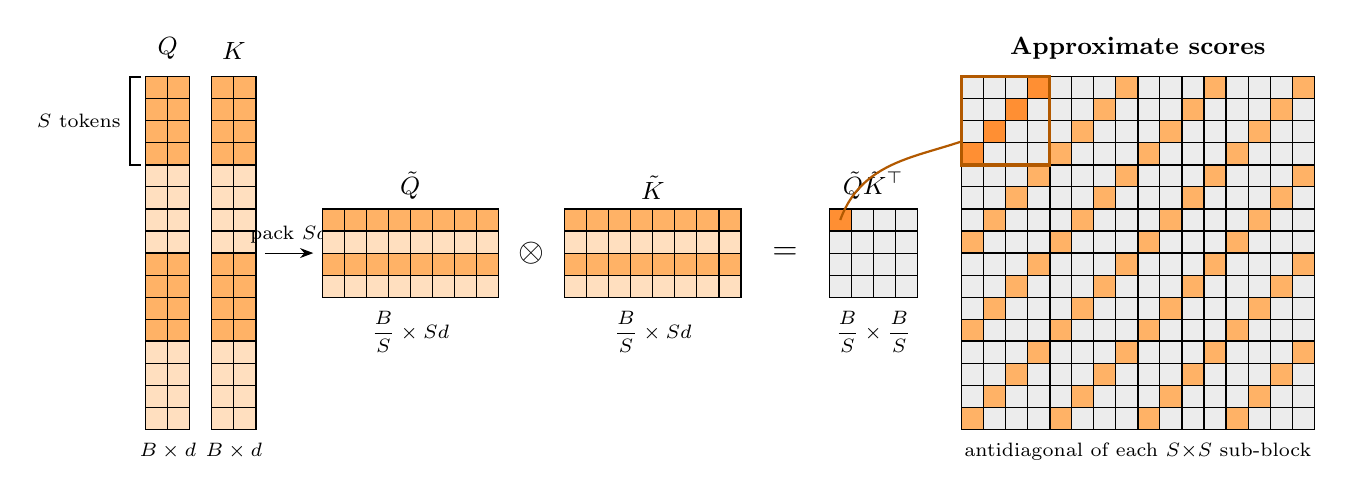
\begin{tikzpicture}
  \def\cell{0.28}
  \colorlet{hilightA}{orange!60}
  \colorlet{hilightB}{orange!25}
  \colorlet{hilightFocus}{orange!90!red!80}
  \colorlet{plain}{gray!15}

  %--- Stride bracket on left of Q ---
  \draw[thick] ({-0.2*\cell},0) -- ({-0.7*\cell},0)
               -- ({-0.7*\cell},{-4*\cell})
               -- ({-0.2*\cell},{-4*\cell});
  \node[left, font=\scriptsize] at ({-0.7*\cell},{-2*\cell}) {$S$ tokens};

  %--- Full Q (16×2, alternating group colours) ---
  \foreach \r in {0,...,15} {
    \pgfmathtruncatemacro{\grp}{mod(int(\r/4),2)}
    \foreach \c in {0,1} {
      \ifnum\grp=0 \fill[hilightA] \else \fill[hilightB] \fi
        ({\c*\cell},{-\r*\cell}) rectangle ({(\c+1)*\cell},{(-\r-1)*\cell});
      \draw ({\c*\cell},{-\r*\cell}) rectangle ({(\c+1)*\cell},{(-\r-1)*\cell});
    }
  }
  \foreach \g in {4,8,12} { \draw[thick] (0,{-\g*\cell}) -- ({2*\cell},{-\g*\cell}); }
  \node[above, font=\small\bfseries] at ({1*\cell}, 0.1)             {$Q$};
  \node[below, font=\scriptsize]     at ({1*\cell},{-16*\cell-0.05}) {$B \times d$};

  %--- Full K (16×2) ---
  \foreach \r in {0,...,15} {
    \pgfmathtruncatemacro{\grp}{mod(int(\r/4),2)}
    \foreach \c in {0,1} {
      \ifnum\grp=0 \fill[hilightA] \else \fill[hilightB] \fi
        ({(3+\c)*\cell},{-\r*\cell}) rectangle ({(4+\c)*\cell},{(-\r-1)*\cell});
      \draw ({(3+\c)*\cell},{-\r*\cell}) rectangle ({(4+\c)*\cell},{(-\r-1)*\cell});
    }
  }
  \foreach \g in {4,8,12} { \draw[thick] ({3*\cell},{-\g*\cell}) -- ({5*\cell},{-\g*\cell}); }
  \node[above, font=\small\bfseries] at ({4*\cell}, 0.1)             {$K$};
  \node[below, font=\scriptsize]     at ({4*\cell},{-16*\cell-0.05}) {$B \times d$};

  %--- Pack arrow ---
  \draw[-{Stealth}] ({5.4*\cell},{-8*\cell}) -- ({7.6*\cell},{-8*\cell});
  \node[above, font=\scriptsize] at ({6.5*\cell},{-8*\cell}) {pack $Sd$};

  %--- Q̃ (4 rows × 8 cols) centred at rows 6–9 ---
  \foreach \r in {0,...,3} {
    \pgfmathtruncatemacro{\grp}{mod(\r,2)}
    \foreach \c in {0,...,7} {
      \ifnum\grp=0 \fill[hilightA] \else \fill[hilightB] \fi
        ({(8+\c)*\cell},{-(6+\r)*\cell}) rectangle ({(9+\c)*\cell},{-(7+\r)*\cell});
      \draw ({(8+\c)*\cell},{-(6+\r)*\cell}) rectangle ({(9+\c)*\cell},{-(7+\r)*\cell});
    }
  }
  \node[above, font=\small\bfseries] at ({12*\cell},{-6*\cell})       {$\tilde{Q}$};
  \node[below, font=\scriptsize]     at ({12*\cell},{-10*\cell-0.05}) {$\dfrac{B}{S} \times Sd$};

  %--- ⊗ ---
  \node[font=\large] at ({17.5*\cell},{-8*\cell}) {$\otimes$};

  %--- K̃ (4 rows × 8 cols) ---
  \foreach \r in {0,...,3} {
    \pgfmathtruncatemacro{\grp}{mod(\r,2)}
    \foreach \c in {0,...,7} {
      \ifnum\grp=0 \fill[hilightA] \else \fill[hilightB] \fi
        ({(19+\c)*\cell},{-(6+\r)*\cell}) rectangle ({(20+\c)*\cell},{-(7+\r)*\cell});
      \draw ({(19+\c)*\cell},{-(6+\r)*\cell}) rectangle ({(20+\c)*\cell},{-(7+\r)*\cell});
    }
  }
  \node[above, font=\small\bfseries] at ({23*\cell},{-6*\cell})       {$\tilde{K}$};
  \node[below, font=\scriptsize]     at ({23*\cell},{-10*\cell-0.05}) {$\dfrac{B}{S} \times Sd$};

  %--- = ---
  \node[font=\large] at ({29*\cell},{-8*\cell}) {$=$};

  %--- 4×4 result matrix (B/S × B/S), centred at rows 6–9 ---
  \foreach \r in {0,...,3} {
    \foreach \c in {0,...,3} {
      \ifnum\r=0
        \ifnum\c=0
          \fill[hilightFocus]
            ({(31+\c)*\cell},{-(6+\r)*\cell}) rectangle ({(32+\c)*\cell},{-(7+\r)*\cell});
        \else
          \fill[plain]
            ({(31+\c)*\cell},{-(6+\r)*\cell}) rectangle ({(32+\c)*\cell},{-(7+\r)*\cell});
        \fi
      \else
        \fill[plain]
          ({(31+\c)*\cell},{-(6+\r)*\cell}) rectangle ({(32+\c)*\cell},{-(7+\r)*\cell});
      \fi
      \draw ({(31+\c)*\cell},{-(6+\r)*\cell}) rectangle ({(32+\c)*\cell},{-(7+\r)*\cell});
    }
  }
  \node[above, font=\small\bfseries] at ({33*\cell},{-6*\cell})       {$\tilde{Q}\tilde{K}^\top$};
  \node[below, font=\scriptsize]     at ({33*\cell},{-10*\cell-0.05}) {$\dfrac{B}{S} \times \dfrac{B}{S}$};

  %--- Arrow from cell (0,0) of 4×4 to sub-block (0,0) of 16×16 ---
  \draw[-{Stealth}, thick, orange!70!black]
      ({31.5*\cell},{-6.5*\cell})
      to[out=70, in=210]
      ({39*\cell},{-2*\cell});

  %--- 16×16 full matrix (cols 37–52, rows 0–15) ---
  \foreach \r in {0,...,15} {
    \foreach \c in {0,...,15} {
      \pgfmathtruncatemacro{\ad}{\r+\c}
      \pgfmathtruncatemacro{\rem}{mod(\ad,4)}
      \pgfmathtruncatemacro{\inblock}{(\r<4)*(\c<4)}
      \ifnum\rem=3
        \ifnum\inblock=1
          \fill[hilightFocus]
        \else
          \fill[hilightA]
        \fi
      \else
        \fill[plain]
      \fi
        ({(37+\c)*\cell},{-\r*\cell}) rectangle ({(38+\c)*\cell},{(-\r-1)*\cell});
      \draw ({(37+\c)*\cell},{-\r*\cell}) rectangle ({(38+\c)*\cell},{(-\r-1)*\cell});
    }
  }
  %--- S×S sub-block grid lines ---
  \foreach \g in {4,8,12} {
    \draw[thick] ({37*\cell},{-\g*\cell}) -- ({53*\cell},{-\g*\cell});
    \draw[thick] ({(37+\g)*\cell},0)      -- ({(37+\g)*\cell},{-16*\cell});
  }
  %--- Outline the focused sub-block (0,0) ---
  \draw[very thick, orange!70!black] ({37*\cell},0) rectangle ({41*\cell},{-4*\cell});

  \node[above, font=\small\bfseries] at ({45*\cell}, 0.1)             {Approximate scores};
  \node[below, font=\scriptsize]     at ({45*\cell},{-16*\cell-0.05}) {antidiagonal of each $S{\times}S$ sub-block};

\end{tikzpicture}
}
\caption{XAttention antidiagonal scoring. Groups of $S$ consecutive tokens are packed along the head dimension ($d \to Sd$), with $K$ groups reversed. Each entry of the $(B/S)\times(B/S)$ product $\tilde{Q}\tilde{K}^\top$ sums the $S$ antidiagonal scores of one $S\times S$ sub-block (arrow).}
\label{fig:xattention_antidiag}
\end{figure}
%% ---- end diagrams/xattention_antidiag ----

The tile scores are normalized with softmax across all key blocks for each query block, producing tile weights. Tiles are then selected greedily in decreasing order of weight until the cumulative weight exceeds a threshold $p$ (top-$p$ selection), yielding a binary mask over the $\lceil N/B \rceil \times \lceil N/B \rceil$ grid of tiles. The threshold $p$ is tuned per attention head.

Since tile scores are a proxy for true attention mass, $p$ cannot be set analytically; the same $p$ value would retain different fractions of true mass in different heads. XAttention calibrates $p$ independently per head: a small set of sample sequences is run through the model, and for each head $p$ is chosen so that the selected tiles cover a target fraction $r$ of the true attention mass (XAttention sets $r=0.9$, corresponding to 90\% recall). XAttention reports results at stride $S=8$ and $S=16$, each with a $32 \times 32$ calibrated threshold table covering all layers and heads.

% ==================== observations ====================
\section{Observations}
\label{sec:observations}

\subsection{Key Similarity}

High cosine similarity between adjacent key states has been observed and studied in KVMerger~\citep{wang2024kvmerger}.
They derive a theoretical lower bound on the cosine similarity between key vectors at positions $n$ and $m$ of $\cos(n - m)$, which puts the minimum similarity of any adjacent pair at $\cos(1) \approx 0.54$.
As the distance between tokens grows, the bound decreases toward zero.
Since this pattern does not appear in value states, they attribute the phenomenon entirely to RoPE.

In this section we look at the pre-RoPE key states to check whether other factors also contribute.
We feed LLaMA-3.1 8B Instruct a sequence of 512 tokens sampled from WikiText-103 and record key states at layers 0, 8, 16, and 23.
At each layer we compute the average cosine similarity between all adjacent token pairs and average over heads.
We repeat this for five configurations:

\begin{enumerate}
    \item \textbf{pre-RoPE real}: key states before RoPE, original token order
    \item \textbf{pre-RoPE shuffled}: key states before RoPE, token positions randomly shuffled
    \item \textbf{post-RoPE real}: key states after RoPE, original token order
    \item \textbf{post-RoPE content shuffled}: key states after RoPE, with the input tokens shuffled before keys are computed
    \item \textbf{post-RoPE shuffled}: key states after RoPE, with the resulting key vectors shuffled afterward
\end{enumerate}

Comparing the shuffled and natural orders lets us isolate the source of the similarity. If the shuffled version drops in cosine similarity, then the natural context order is contributing to the phenomenon, since shuffling is the only thing that changed. If it stays high, the similarity comes from something other than content order. We also compare pre-RoPE and post-RoPE states to separate out the effect of RoPE, and we shuffle either the input content or the final key vectors to tell apart content-driven adjacency from positional adjacency.

%% ---- begin diagrams/key_similarity_bars ----
\begin{figure}[!ht]
\centering
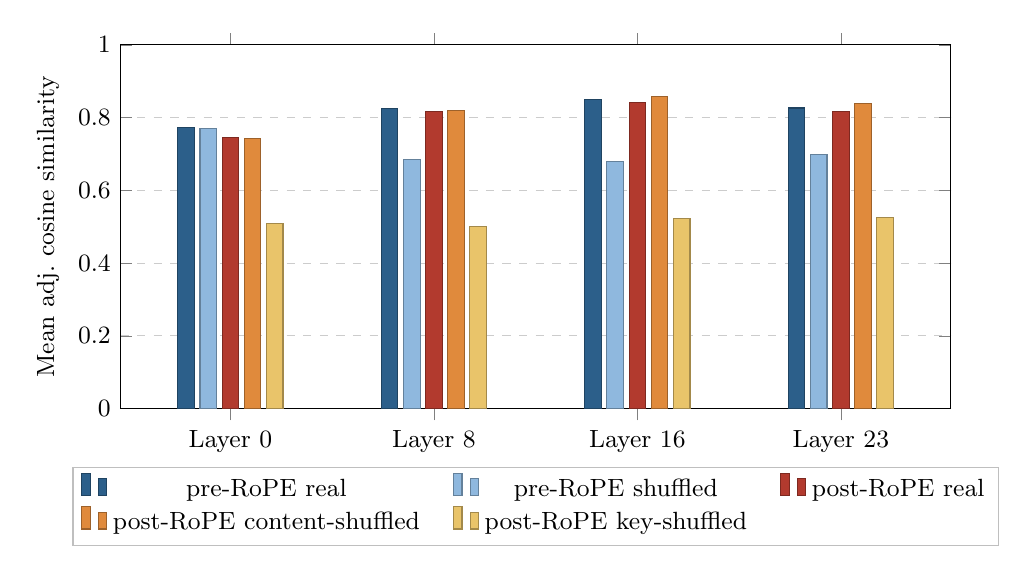
\begin{tikzpicture}
  \definecolor{preReal}{HTML}{2C5F8A}   % dark blue
  \definecolor{preShuf}{HTML}{8FB8DE}   % light blue
  \definecolor{postReal}{HTML}{B23A2E}  % dark red
  \definecolor{postCont}{HTML}{E08A3C}  % orange
  \definecolor{postShuf}{HTML}{E9C46A}  % light amber
  \begin{axis}[
    ybar,
    bar width=6pt,
    width=\textwidth,
    height=6.2cm,
    enlarge x limits=0.18,
    ymin=0, ymax=1,
    ytick={0,0.2,0.4,0.6,0.8,1.0},
    ylabel={Mean adj.\ cosine similarity},
    symbolic x coords={Layer 0, Layer 8, Layer 16, Layer 23},
    xtick=data,
    tick label style={font=\small},
    ylabel style={font=\small},
    ymajorgrids=true,
    grid style={dashed, gray!40},
    legend style={
      at={(0.5,-0.16)}, anchor=north,
      legend columns=3, font=\small,
      /tikz/every even column/.append style={column sep=10pt},
      draw=gray!50,
    },
  ]
    \addplot[fill=preReal,  draw=preReal!70!black]  coordinates {(Layer 0,0.7728) (Layer 8,0.8252) (Layer 16,0.8498) (Layer 23,0.8264)};
    \addplot[fill=preShuf,  draw=preShuf!70!black]  coordinates {(Layer 0,0.7700) (Layer 8,0.6837) (Layer 16,0.6806) (Layer 23,0.6989)};
    \addplot[fill=postReal, draw=postReal!70!black] coordinates {(Layer 0,0.7457) (Layer 8,0.8167) (Layer 16,0.8423) (Layer 23,0.8172)};
    \addplot[fill=postCont, draw=postCont!70!black] coordinates {(Layer 0,0.7434) (Layer 8,0.8200) (Layer 16,0.8573) (Layer 23,0.8390)};
    \addplot[fill=postShuf, draw=postShuf!70!black] coordinates {(Layer 0,0.5094) (Layer 8,0.5005) (Layer 16,0.5216) (Layer 23,0.5242)};
    \legend{pre-RoPE real, pre-RoPE shuffled, post-RoPE real, post-RoPE content-shuffled, post-RoPE key-shuffled}
  \end{axis}
\end{tikzpicture}
\caption{Average cosine similarity of adjacent key states under five configurations for LLaMA-3.1 8B Instruct at layers 0, 8, 16, and 23.}
\label{fig:cos_analysis}
\end{figure}
%% ---- end diagrams/key_similarity_bars ----

The pre-RoPE shuffled configuration in Figure~\ref{fig:cos_analysis} already shows high cosine similarity.
Since the token order is random here, neither positional encoding nor content adjacency can explain it.
The key projection itself pushes key states into a narrow region of the key space, raising the global similarity.
This is the structure that low-rank KV compression methods exploit, such as EigenAttention~\citep{saxena2024eigenattention} and DeepSeek MLA~\citep{deepseekai2024deepseekv2}.

In mid and deep layers, the pre-RoPE real configuration in Figure~\ref{fig:cos_analysis} shows noticeably higher similarity than pre-RoPE shuffled.
Adjacent tokens in natural text tend to be semantically related, and this is reflected in their key states.

Comparing the pre-RoPE real and post-RoPE real configurations in Figure~\ref{fig:cos_analysis}, the similarity values are nearly identical.
When content is in natural order, applying RoPE does not significantly change adjacent token similarity.

The post-RoPE content-shuffled configuration in Figure~\ref{fig:cos_analysis} shows a different picture.
The input content is shuffled before keys are computed, so the key states lack content-driven adjacency.
After RoPE is applied, the similarity recovers to nearly the level of post-RoPE real.
RoPE raises the similarity of adjacent positions regardless of the underlying content order.

The post-RoPE key-shuffled configuration in Figure~\ref{fig:cos_analysis} shows what happens if we break positional adjacency after RoPE is applied. The similarity drops back down, confirming that RoPE's contribution relies on evaluating adjacent positions sequentially.

Key similarity at the token level is therefore a combination of three factors: the key projection creates a high global similarity floor, semantic content raises similarity further for adjacent tokens in natural text, and RoPE contributes a positional adjacency structure on top of that.

\subsection{Query Similarity}

The same analysis on query states shows that the query projection has the same properties as the key projection.
Query vectors show high cosine similarity regardless of token order, which means the projection itself pushes queries into a narrow region of the query space.
In later layers, similarity is higher for real sequences than for shuffled ones, suggesting that query vectors pick up contextual information and adjacent tokens in natural text end up closer together.
As with keys, applying RoPE to shuffled sequences (post-RoPE content-shuffled) recovers adjacent similarity, contributing a positional structure on top of the content signal. Furthermore, breaking the positional adjacency after RoPE (post-RoPE Q-shuffled) drops the similarity back down.

%% ---- begin diagrams/query_similarity_bars ----
\begin{figure}[!ht]
\centering
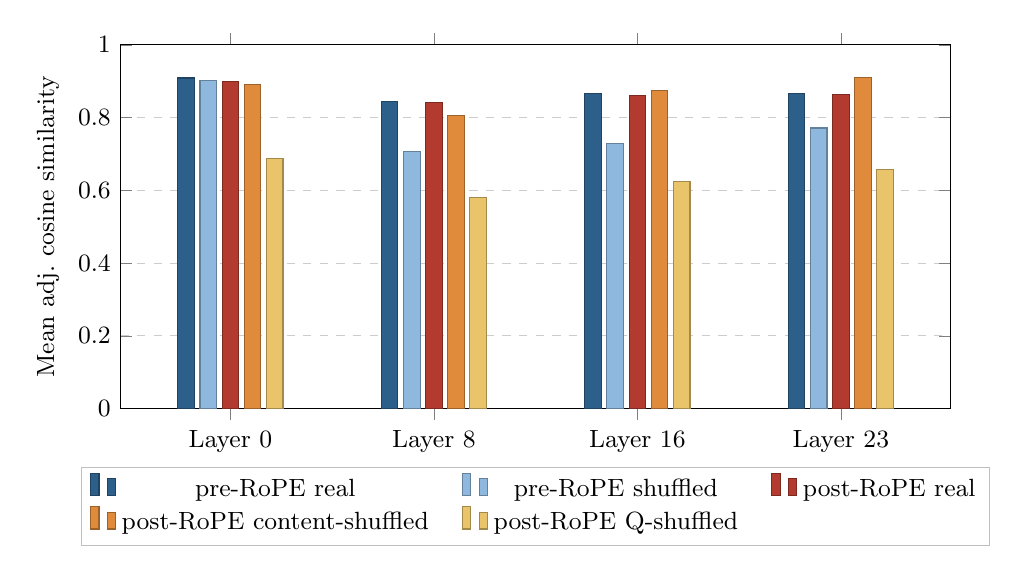
\begin{tikzpicture}
  \definecolor{preReal}{HTML}{2C5F8A}   % dark blue
  \definecolor{preShuf}{HTML}{8FB8DE}   % light blue
  \definecolor{postReal}{HTML}{B23A2E}  % dark red
  \definecolor{postCont}{HTML}{E08A3C}  % orange
  \definecolor{postShuf}{HTML}{E9C46A}  % light amber
  \begin{axis}[
    ybar,
    bar width=6pt,
    width=\textwidth,
    height=6.2cm,
    enlarge x limits=0.18,
    ymin=0, ymax=1,
    ytick={0,0.2,0.4,0.6,0.8,1.0},
    ylabel={Mean adj.\ cosine similarity},
    symbolic x coords={Layer 0, Layer 8, Layer 16, Layer 23},
    xtick=data,
    tick label style={font=\small},
    ylabel style={font=\small},
    ymajorgrids=true,
    grid style={dashed, gray!40},
    legend style={
      at={(0.5,-0.16)}, anchor=north,
      legend columns=3, font=\small,
      /tikz/every even column/.append style={column sep=10pt},
      draw=gray!50,
    },
  ]
    \addplot[fill=preReal,  draw=preReal!70!black]  coordinates {(Layer 0,0.9091) (Layer 8,0.8449) (Layer 16,0.8652) (Layer 23,0.8659)};
    \addplot[fill=preShuf,  draw=preShuf!70!black]  coordinates {(Layer 0,0.9010) (Layer 8,0.7075) (Layer 16,0.7281) (Layer 23,0.7716)};
    \addplot[fill=postReal, draw=postReal!70!black] coordinates {(Layer 0,0.9000) (Layer 8,0.8408) (Layer 16,0.8619) (Layer 23,0.8626)};
    \addplot[fill=postCont, draw=postCont!70!black] coordinates {(Layer 0,0.8922) (Layer 8,0.8047) (Layer 16,0.8736) (Layer 23,0.9114)};
    \addplot[fill=postShuf, draw=postShuf!70!black] coordinates {(Layer 0,0.6880) (Layer 8,0.5807) (Layer 16,0.6234) (Layer 23,0.6570)};
    \legend{pre-RoPE real, pre-RoPE shuffled, post-RoPE real, post-RoPE content-shuffled, post-RoPE Q-shuffled}
  \end{axis}
\end{tikzpicture}
\caption{Mean adjacent query cosine similarity per layer (averaged over all heads) for LLaMA-3.1 8B Instruct at layers 0, 8, 16, and 23, under five configurations: pre-RoPE real, pre-RoPE shuffled, post-RoPE real, post-RoPE content-shuffled, and post-RoPE Q-shuffled.}
\label{fig:query_similarity}
\end{figure}
%% ---- end diagrams/query_similarity_bars ----

% ==================== related_work ====================
\section{Related Work}

\paragraph{Attention complexity and FlashAttention.}
Self-attention scales quadratically in both time and memory with sequence length, which made long-context inference impractical for early Transformer models.
FlashAttention~\citep{dao2022flashattention} addressed the memory side by computing attention in tiles in on-chip SRAM, avoiding materializing the full attention matrix in HBM.
This brought memory use down to linear and cut HBM traffic substantially, making attention practical for sequences up to tens of thousands of tokens.
However, FlashAttention is exact (every attention score is still computed), so the quadratic time complexity remains.
As sequences grow attention computation becomes the dominant runtime cost and approximate methods become necessary.

\paragraph{Sparse attention for prefill.}
A natural way to reduce the time cost is to exploit the fact that attention matrices are empirically sparse: most tokens attend strongly to only a small fraction of others.
\citet{child2019generating} were among the first to demonstrate this, observing that trained Transformer attention matrices concentrate on local windows and a few distant positions.
They proposed fixed sparse patterns (local windows combined with strided or fixed summary positions) to approximate full attention with fewer FLOPs.
The limitation is that a fixed pattern cannot adapt to the content of a given input. This motivated a shift to dynamic sparse attention, where the sparsity pattern is determined on the fly. These methods generally fall into two categories: attention shape methods and block-sparse attention methods.

\textbf{Block-sparse attention methods} dynamically skip attention tiles that are estimated to be unimportant. SpargeAttn~\citep{zhang2025spargeattn} selects a representative per block using mean pooling and scores tiles based on the block representatives. XAttention~\citep{xu2025xattention} uses the sum of antidiagonal values within each attention block as a lightweight proxy for tile importance. Both methods then compute attention only for the tiles scored as important.

\textbf{Attention shape methods} in contrast identify the attention pattern a head exhibits and exploit it. MInference~\citep{jiang2024minference}, a foundational paper in the field, widely used in production, found that LLM attention heads follow consistent structural patterns across different inputs (A-shape, Vertical-Slash, and Block-Sparse). It assigns each head its dominant pattern offline and builds sparse indices at inference time accordingly. Crucially, Block-Sparse heads do not fit the A-shape or Vertical-Slash patterns, so there is no fixed shape to exploit. For these heads MInference falls back to block-sparse attention: it mean-pools each query and key block into a single representative, then uses the representative-level attention scores to pick the important tiles, in the same way as SpargeAttn.

FlexPrefill~\citep{lai2025flexprefill} extends MInference by making it content-adaptive. Instead of assigning a shape to a head offline, FlexPrefill decides at inference time whether to treat a head as Vertical-Slash or block-sparse, based on the Jensen-Shannon divergence between the head's attention and each candidate pattern. It also differs in how tiles are selected. MInference uses top-k selection, keeping the best $k$ blocks and tokens, while FlexPrefill uses top-p selection, keeping blocks and tokens until they hold $p\%$ of the attention mass. FlexPrefill defaults to $p=90$, so the selected blocks and tokens are expected to hold 90 percent of the attention mass.


As a parallel line, \citet{qi2024deltallm}, a concurrent work from our group at LIACS, targets a different kind of sparsity.
While the methods above exploit the empirical sparsity of the attention map, they observe that adjacent key vectors are similar, so encoding each key as a delta from the previous one yields a sparse delta key matrix.
They then propose a method to compute attention directly using this delta key matrix, reducing the overall computation.
However, the delta is applied element-wise, giving unstructured sparsity scattered throughout the delta matrix, a pattern that GPU hardware cannot exploit efficiently, requiring custom hardware to accelerate.

\paragraph{KV cache compression for decoding.}
A separate line of work targets the memory bottleneck of autoregressive decoding.
KVMerger~\citep{wang2024kvmerger} observed that adjacent token embeddings in the key matrix exhibit high cosine similarity within a sequence, and that this pattern is consistent across datasets and layers. This motivates merging consecutive similar key tokens into a single representative, compressing the KV cache without throwing away information.

\paragraph{Delta-based prefill acceleration.}
The three methods in this thesis are all training-free prefill acceleration methods built on a single observation: adjacent tokens have highly similar key and query vectors.
Each method applies this insight in a different setting, and each has a different closest relative among the methods above.

Delta-KV compression is a direct prefill optimization and is closest to KVMerger~\citep{wang2024kvmerger}.
Both compress the KV by merging adjacent keys that are nearly identical.
KVMerger does this to shrink the KV cache for decoding, while we compress $K$ at prefill to cut the cost of the $QK$ multiplication.

DeltaXAttention asks whether the delta principle can be layered on top of an existing block-sparse method rather than used on its own.
We take XAttention~\citep{xu2025xattention} and apply delta compression to the keys inside the tiles it selects, compressing within each tile on top of the tiles XAttention already skips.

Delta-based tile scoring (DPXA) is closest to XAttention~\citep{xu2025xattention} and SpargeAttn~\citep{zhang2025spargeattn}.
All three compute a cheap importance score for each tile to decide which tiles to compute exactly.
XAttention sums the antidiagonal values of each block, and SpargeAttn mean-pools each block into a single representative. DPXA, however, compresses $Q$ and $K$ to perform a lightweight attention that represents the tile's importance. Unlike XAttention, which relies on rigid strides, DPXA's tile scoring is fully content-adaptive, thereby avoiding the risk of missing critical information.

% ==================== methodology ====================
\section{Methodology}

This section describes the three methods. We first introduce Delta-KV compression, the core mechanism that compresses the key and value matrices before attention (Section~\ref{sec:delta_kv}). We then layer this mechanism on top of a block-sparse method to give DeltaXAttention (Section~\ref{sec:xattention_adaptation}), and finally repurpose it as a tile importance estimator for delta-based tile scoring (Section~\ref{sec:delta_tile_scoring}).

\subsection{Delta-KV Compression}
\label{sec:delta_kv}

\begin{figure}[!ht]
    \centering
    
\includegraphics[width=0.65\textwidth]{assets/delta_attention.jpeg}
    \caption{The three stages of Delta-KV compression. Stage 1 (pre-processing) computes row-wise deltas of $K$ and thresholds them into a keep mask. Stage 2 (packing) drops the masked rows to form $\hat{K}$ and $\hat{V}$ of length $m < n$. Stage 3 (self-attention) multiplies $Q$ against $\hat{K}$, applies softmax, and multiplies by $\hat{V}$ to give the $n \times l$ output.}
    \label{fig:delta_attention}
\end{figure}

Delta-KV compression operates in three stages: pre-processing analyzes the key matrix to identify which rows to keep, packing compresses the KV matrices based on the retained rows, and self-attention computes the output against the compressed matrices. We then adapt FlashAttention-2 to work on these compressed KV matrices to realize end-to-end speedups on long-context tasks.

\subsubsection{Stage 1: Pre-processing}
\label{sec:preprocessing}

The pre-processing stage takes the key matrix $K$ as input and outputs a binary keep mask of length $n$. It analyzes $K$ row by row to decide which rows to keep (which we refer to as \textbf{anchors}) and which to drop (steps 1.1 and 1.2 in Figure~\ref{fig:delta_attention}).

We initialize a keep mask of length $n$ to all ones, meaning all rows are initially kept. The anchor is set to the first row $K_0$. We then iterate over the remaining rows:

\begin{enumerate}
    \item Compute the distance or similarity $\delta_i$ (e.g., Euclidean distance or cosine similarity) between row $K_i$ and the current anchor:
    \begin{equation}
        \delta_i = \text{metric}(K_i, \text{anchor})
    \end{equation}
    \item If $\delta_i$ indicates the row is sufficiently different from the anchor for a given threshold $\tau$ (e.g., $\delta_i > \tau$ for Euclidean distance, or $\delta_i < \tau$ for cosine similarity), we keep it and move the anchor to $K_i$.
    \item Otherwise, the row is similar enough that the anchor can represent it, so we drop it by setting $\text{keepmask}[i] = 0$ and leave the anchor unchanged.
\end{enumerate}

The output keep mask has a 1 at each anchor position and a 0 at each dropped position.

Crucially, the sequential comparison is performed over chunks of 512 tokens. The sequence is divided into non-overlapping chunks and each chunk is processed in parallel. The first token of each chunk is treated as an anchor, which breaks the sequential dependency between chunks and allows them to be processed in parallel.

\subsubsection{Stage 2: Packing}
\label{sec:packing}

The packing stage takes the keep mask from stage 1 as input and outputs compressed key and value matrices $\hat{K}$ and $\hat{V}$, and a vector $\text{packed\_counts}$ (step 2.1 in Figure~\ref{fig:delta_attention}).

We drop all rows of $K$ and $V$ where the keep mask is 0, keeping only the anchor rows. The resulting $\hat{K}$ and $\hat{V}$ have shape $m \times l$, where $m < n$ is the number of anchors.

We also compute $\text{packed\_counts}$ of length $m$, where $\text{packed\_counts}[j]$ is the run length of anchor $j$, the number of rows it represents including itself.

\subsubsection{Stage 3: Self-Attention}
\label{sec:self_attention_compressed}

The final stage takes the original query matrix $Q$ and the packed matrices $\hat{K}$, $\hat{V}$, and $\text{packed\_counts}$ from stage 2 as input, and outputs the attention output of shape $n \times l$. It follows the same steps as standard self-attention (Section~\ref{sec:self_attention}), with two differences: $Q$ is multiplied against the compressed $\hat{K}$ and $\hat{V}$ instead of the full matrices, and the softmax is weighted by $\text{packed\_counts}$.

\begin{enumerate}
    \item \textbf{Attention scores} (step 3.1): Multiply $Q$ by $\hat{K}^\top$ to get the score matrix:
    \begin{equation}
        S = \frac{Q\hat{K}^\top}{\sqrt{l}}
    \end{equation}
    $S$ has shape $n \times m$, where entry $(i, j)$ encodes how much token $i$ attends to anchor $j$.

    \item \textbf{Count-weighted softmax} (step 3.2): An anchor representing many tokens should have a proportionally larger effect than one representing a single token. To account for this, we scale each column of $S$ by the corresponding entry in $\text{packed\_counts}$ before applying the softmax:
    \begin{equation}
        \label{eq:count_weighted_softmax}
        W_{i,j} = \frac{\text{packed\_counts}[j] \cdot \exp(S_{i,j})}{\displaystyle\sum_{k=1}^{m} \text{packed\_counts}[k] \cdot \exp(S_{i,k})}
    \end{equation}
    For example, if token $i$ attends to anchor $j$ with score 5 and anchor $j$ represents 10 tokens, its unnormalized softmax weight $\exp(5)$ is scaled by 10 before normalization. This is equivalent to running standard self-attention where the anchor key vector is copied to all token positions it represents.

    \item \textbf{Attention output} (step 3.3): Multiply the attention weights by the packed value matrix:
    \begin{equation}
        \text{output} = W\hat{V}
    \end{equation}
    The compressed sequence dimension $m$ disappears after this multiplication, giving an output of shape $n \times l$, identical in shape to the output of standard self-attention.
\end{enumerate}

\subsubsection{FlashAttention Adaptation}
\label{sec:flash_attention_adaptation}

To test Delta-KV compression on long context tasks we modified FlashAttention-2 to operate on the compressed $\hat{K}$ and $\hat{V}$ matrices. The kernel follows the same structure as FlashAttention-2 (Section~\ref{sec:flashattention_algorithm}): an outer loop over query blocks, with each kernel program handling one query block independently. The inner loop is modified to operate in two phases.

Alongside $\hat{K}$, $\hat{V}$, and $\text{packed\_counts}$, we store a $\texttt{packed\_timestamps}$ vector of length $m$. Entry $j$ holds the index in the original sequence of the last token that anchor $j$ represents. For example, if anchor $j$ represents tokens 5, 6, and 7 from the original sequence, then $\texttt{packed\_timestamps}[j] = 7$. This vector can be computed as a cumulative sum of $\text{packed\_counts}$, minus one. It lets the kernel track how far into the original sequence each anchor's coverage extends.

\textbf{Phase 1: Compressed history.} The first phase iterates over blocks of $\hat{K}$ and $\hat{V}$ instead of blocks of $K$. For each packed block, the kernel reads the $\texttt{packed\_timestamps}$ of the anchors in that block and takes their maximum. This is the reach of the block: the furthest position in the original sequence that any anchor in the block represents.

We define the \textbf{critical diagonal} of a query block as the span of positions the block itself covers, $[\text{query\_block\_start},\, \text{query\_block\_end}]$. Any key anchor whose reach falls within this span represents tokens that overlap with the current query block and must be processed exactly. This follows the local attention window principle described in Section~\ref{sec:local_attention_window}: tokens attend most strongly to their immediate neighbors, so those neighbors must be kept exact.

If the reach falls before the critical diagonal (reach $<$ query\_block\_start), the block is safe to process in compressed form. The kernel computes the attention scores against the packed key vectors and applies count-weighted softmax exactly as in Equation~\ref{eq:count_weighted_softmax}, updating the online softmax running state ($m_i$, $l_i$, $\text{acc}$) as in standard FlashAttention.

If the reach falls inside or past the critical diagonal, the first phase stops. Those anchors cover tokens that belong to the current query block, so they need to be processed exactly.

\textbf{Phase 2: Critical diagonal.} The second phase switches to the original uncompressed $K$ and $V$. Starting from just after the last safe anchor's reach and going up to the end of the current query block, it runs standard FlashAttention over the exact token vectors.

\subsection{DeltaXAttention}
\label{sec:xattention_adaptation}

Block-sparse attention methods such as XAttention~\citep{xu2025xattention} and SpargeAttention~\citep{zhang2025spargeattn} are orthogonal to Delta-KV compression: one reduces the number of tiles computed, the other reduces the cost of each tile. The two can be combined to decrease both computation and data movement. We implement Delta-KV compression on top of XAttention, a strong recent block-sparse prefill method, and call the result DeltaXAttention.

XAttention produces a binary tile mask before the attention computation (Section~\ref{sec:xattention}). For tiles the mask selects, the standard approach loads the full uncompressed $K$ and $V$ blocks. In our adaptation, we instead load the compressed $\hat{K}$ and $\hat{V}$ blocks and compute the attention output using count-weighted softmax as described in Section~\ref{sec:self_attention_compressed}.
\subsubsection{Preserving accuracy}

Using packed KV for all non-skipped tiles hurts accuracy. The source of this degradation is the diagonal tiles. As established in Section~\ref{sec:local_attention_window}, diagonal tiles correspond to local attention between neighboring tokens and carry the most attention mass. Substituting compressed keys for these tiles introduces approximation error where the model is most sensitive.

To address this, we never apply delta compression to diagonal tiles. They are always computed using the full uncompressed $K$ and $V$.

For off-diagonal tiles, we additionally keep the top 10\% by XAttention tile importance score exact, computing them with full $K$ and $V$ as well. The remaining off-diagonal tiles use the packed $\hat{K}$ and $\hat{V}$.

We measure the effect of this approach using a KV reduction metric computed per attention head. KV reduction is the decrease in total KV loads relative to standard XAttention. If a fraction $f$ of tiles are computed with packed KV and the packing reduces those KV matrices to a fraction $p$ of their original size, then the KV reduction is $f(1-p)$. For example, if half the tiles use packed KV and delta packing halves the KV size, the KV reduction is $0.5 \times 0.5 = 25\%$.

\subsubsection{Ablation}
\label{sec:xattention_ablation}

XAttention natively can also reduce KV loads without delta compression by simply skipping more tiles. Concretely, for a target KV reduction of $\alpha$\%, we skip the $\alpha$\% least important off-diagonal tiles that XAttention would otherwise compute. This gives the same KV reduction as a DeltaXAttention configuration tuned to $\alpha$\%, but through tile skipping alone rather than key compression.

We compare the two approaches at matched KV reduction. If XAttention tile skipping preserves more accuracy than DeltaXAttention at the same reduction, then applying delta compression on top of XAttention adds no value. This serves as a direct check on whether the combination is meaningful.

\subsection{Delta-Based Tile Scoring (DPXA)}
\label{sec:delta_tile_scoring}

XAttention estimates tile importance by compressing $Q$ and $K$ into $\tilde{Q}$ and $\tilde{K}$ of shape $(B/S) \times Sl$ using a fixed stride $S$ (Section~\ref{sec:xattention}, Figure~\ref{fig:xattention_antidiag}). Groups of $S$ consecutive tokens are concatenated along the head dimension, so the scoring cost is $O(B^2/S)$, a factor of $1/S$ of the full tile. For stride $S=8$ this is $12.5\%$ of full tile cost.

Delta compression offers a content-adaptive alternative. Rather than sampling every $S$-th token by fixed stride, we apply delta pre-processing (Section~\ref{sec:preprocessing}) independently to $Q$ and $K$ to select anchors, giving $Q^\delta$ and $K^\delta$ of shapes $(\alpha B) \times l$ and $(\beta B) \times l$, where $\alpha$ and $\beta$ are the keep ratios of $Q$ and $K$ respectively (Figure~\ref{fig:delta_tile_scoring}). Crucially, no dimension expansion is performed: the head dimension stays at $l$. Their product $Q^\delta {K^\delta}^\top$ has shape $(\alpha B) \times (\beta B)$ and costs a fraction $\alpha \beta$ of the full tile. We call this the \textbf{scoring ratio}. It has a second, equivalent reading: since each entry of $Q^\delta {K^\delta}^\top$ is a single cell of the full $B \times B$ attention tile, $\alpha\beta$ is also the fraction of the tile's cells that are sampled to estimate its importance.

This differs from the XAttention approach in two ways. First, $Q^\delta$ and $K^\delta$ can have different numbers of anchors, since $Q$ and $K$ are compressed independently (Figure~\ref{fig:delta_tile_scoring}). Second, each entry of $Q^\delta {K^\delta}^\top$ corresponds to a single dot product between one $Q$ anchor and one $K$ anchor, a single position in the full $B \times B$ score tile, rather than a sum over an $S \times S$ sub-block as in XAttention.

We summarize the procedure. Each pair of a query block and a key block defines one \textbf{tile}: the $B \times B$ score matrix that full attention would compute for that pair. Step 1 compacts the blocks. Steps 2 and 3 score the tiles. Once all tile scores are available, steps 4 and 5 select the tiles and compute the attention.

\begin{enumerate}
    \item \textbf{Compaction (per block)}: For each query block and each key block, apply delta pre-processing (Stage 1, Section~\ref{sec:preprocessing}) and gather the anchor rows as in packing (Stage 2, Section~\ref{sec:packing}). This gives a compacted $Q^\delta$ of shape $(\alpha B) \times l$ for each query block and $K^\delta$ of shape $(\beta B) \times l$ for each key block, where $\alpha$ and $\beta$ are the per-block keep ratios of $Q$ and $K$. In Figure~\ref{fig:delta_tile_scoring}, the leftmost two matrices show the delta selection that determines the anchors, and the two matrices to their right are the resulting compacted $Q^\delta$ and $K^\delta$. Unlike Stage 2, we do not compute $\text{packed\_counts}$: the anchors serve only as a sampling pattern.

    \item \textbf{Sampled score matrix (per tile)}: For each tile, multiply the compacted query block $Q^\delta$ and key block $K^\delta$ to get the score matrix $Q^\delta {K^\delta}^\top$ of shape $(\alpha B) \times (\beta B)$ (the resulting matrix in Figure~\ref{fig:delta_tile_scoring}). Each entry is a single cell of the full $B \times B$ tile, so this costs a fraction $\alpha \beta$ (the scoring ratio) of the full tile.

    \item \textbf{Tile importance (per tile)}: Exponentiate each entry of the score matrix and sum the results into a single importance score for that tile.

    \item \textbf{Top-$p$ tile selection}: Once every tile has an importance score, normalize the scores of each query block with a softmax across all key blocks to obtain tile weights. For each query block, select tiles in decreasing order of weight until their cumulative weight exceeds the threshold $p$, yielding the binary block mask (Figure~\ref{fig:dpxa_3part}).

    \item \textbf{Attention}: Compute attention over the selected tiles with the standard block-sparse kernel, using the full $Q$, $K$, and $V$ (Figure~\ref{fig:dpxa_3part}).
\end{enumerate}

\textbf{Threshold calibration.} Step 4 selects tiles by top-$p$: for each query block we add tiles in decreasing order of weight until their cumulative weight exceeds the threshold $p$. We set a target recall $r = 0.90$, the fraction of true attention mass each head should retain (the value used by both XAttention and FlexPrefill). Since the tile weights are only a proxy for the true mass, setting $p = r$ would retain a different fraction than $90\%$, so we calibrate $p$ per head offline. On a small set of calibration texts we run full attention and, for each head and query block, sum the exact softmax weights into a true per-tile mass. Ranking tiles by this true mass, we take the smallest set that covers $r$ of it, then read off the cumulative estimator-mass fraction that reproduces exactly that set; this is the top-$p$ value that makes DPXA's proxy scores select the same tiles. This procedure gives a $p$ per query block, which we pool over query blocks into a single $p$ per head. Each calibration text yields a different $p$. For each head we sort its per-text $p$ values and read off the value at the 90th percentile, the point below which $90\%$ of the texts fall, a robust choice that ignores the single most extreme text. This gives one calibrated threshold $p$ per (layer, head), which we load at inference. This calibration follows XAttention (Section~\ref{sec:xattention}), with a single change: we aggregate across calibration sequences with the 90th percentile rather than XAttention's maximum, which is less sensitive to a single outlier sequence.

%% ---- begin diagrams/delta_tile_scoring ----
\begin{figure}[h]
\centering
\resizebox{\textwidth}{!}{
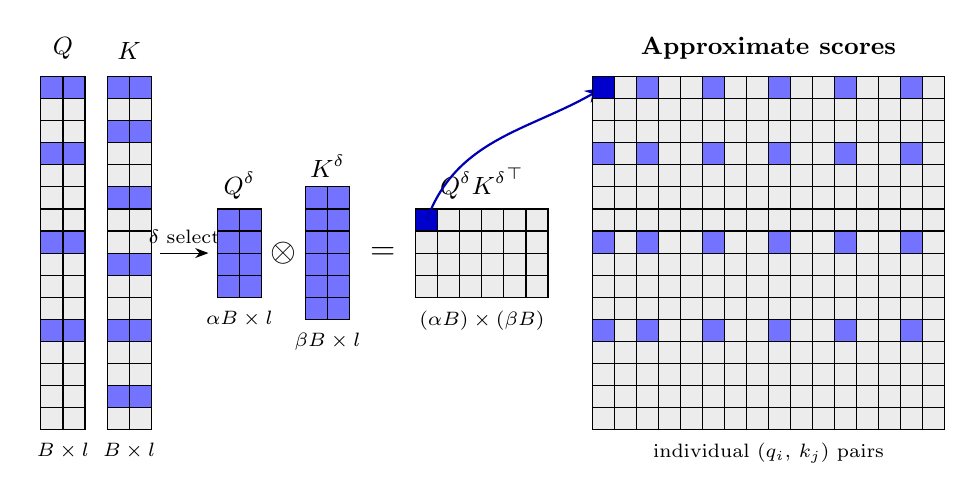
\begin{tikzpicture}
  \def\cell{0.28}
  \colorlet{hilightA}{blue!55}
  \colorlet{hilightFocus}{blue!80!black}
  \colorlet{plain}{gray!15}

  % Q anchors: rows 0, 3, 7, 11   (4 of 16)
  % K anchors: rows 0, 2, 5, 8, 11, 14  (6 of 16)

  %--- Full Q (16 rows × 2 cols) — anchor rows in orange ---
  \foreach \r in {0,...,15} {
    \pgfmathtruncatemacro{\isanchor}{
      (((\r==0)+(\r==3)+(\r==7)+(\r==11))>0) ? 1 : 0
    }
    \foreach \c in {0,1} {
      \ifnum\isanchor=1 \fill[hilightA] \else \fill[plain] \fi
        ({\c*\cell},{-\r*\cell}) rectangle ({(\c+1)*\cell},{(-\r-1)*\cell});
      \draw ({\c*\cell},{-\r*\cell}) rectangle ({(\c+1)*\cell},{(-\r-1)*\cell});
    }
  }
  \node[above, font=\small\bfseries] at ({1*\cell}, 0.1)             {$Q$};
  \node[below, font=\scriptsize]     at ({1*\cell},{-16*\cell-0.05}) {$B \times l$};

  %--- Full K (16 rows × 2 cols) — different anchor pattern ---
  \foreach \r in {0,...,15} {
    \pgfmathtruncatemacro{\isanchor}{
      (((\r==0)+(\r==2)+(\r==5)+(\r==8)+(\r==11)+(\r==14))>0) ? 1 : 0
    }
    \foreach \c in {0,1} {
      \ifnum\isanchor=1 \fill[hilightA] \else \fill[plain] \fi
        ({(3+\c)*\cell},{-\r*\cell}) rectangle ({(4+\c)*\cell},{(-\r-1)*\cell});
      \draw ({(3+\c)*\cell},{-\r*\cell}) rectangle ({(4+\c)*\cell},{(-\r-1)*\cell});
    }
  }
  \node[above, font=\small\bfseries] at ({4*\cell}, 0.1)             {$K$};
  \node[below, font=\scriptsize]     at ({4*\cell},{-16*\cell-0.05}) {$B \times l$};

  %--- Delta-select arrow ---
  \draw[-{Stealth}] ({5.4*\cell},{-8*\cell}) -- ({7.6*\cell},{-8*\cell});
  \node[above, font=\scriptsize] at ({6.5*\cell},{-8*\cell}) {$\delta$ select};

  %--- Q^δ (4 rows × 2 cols, centred at rows 6–9) ---
  \foreach \r in {0,...,3} {
    \foreach \c in {0,1} {
      \fill[hilightA]
        ({(8+\c)*\cell},{-(6+\r)*\cell}) rectangle ({(9+\c)*\cell},{-(7+\r)*\cell});
      \draw ({(8+\c)*\cell},{-(6+\r)*\cell}) rectangle ({(9+\c)*\cell},{-(7+\r)*\cell});
    }
  }
  \node[above, font=\small\bfseries] at ({9*\cell},{-6*\cell})       {$Q^\delta$};
  \node[below, font=\scriptsize]     at ({9*\cell},{-10*\cell-0.05}) {$\alpha B \times l$};

  %--- ⊗ ---
  \node[font=\large] at ({11*\cell},{-8*\cell}) {$\otimes$};

  %--- K^δ (6 rows × 2 cols, centred at rows 5–10) — taller than Q^δ ---
  \foreach \r in {0,...,5} {
    \foreach \c in {0,1} {
      \fill[hilightA]
        ({(12+\c)*\cell},{-(5+\r)*\cell}) rectangle ({(13+\c)*\cell},{-(6+\r)*\cell});
      \draw ({(12+\c)*\cell},{-(5+\r)*\cell}) rectangle ({(13+\c)*\cell},{-(6+\r)*\cell});
    }
  }
  \node[above, font=\small\bfseries] at ({13*\cell},{-5*\cell})       {$K^\delta$};
  \node[below, font=\scriptsize]     at ({13*\cell},{-11*\cell-0.05}) {$\beta B \times l$};

  %--- = ---
  \node[font=\large] at ({15.5*\cell},{-8*\cell}) {$=$};

  %--- (αB)×(βB) result matrix: 4 rows × 6 cols, centred at rows 6–9 ---
  \foreach \r in {0,...,3} {
    \foreach \c in {0,...,5} {
      \pgfmathtruncatemacro{\isFocus}{(\r==0)*(\c==0)}
      \ifnum\isFocus=1
        \fill[hilightFocus]
      \else
        \fill[plain]
      \fi
        ({(17+\c)*\cell},{-(6+\r)*\cell}) rectangle ({(18+\c)*\cell},{-(7+\r)*\cell});
      \draw ({(17+\c)*\cell},{-(6+\r)*\cell}) rectangle ({(18+\c)*\cell},{-(7+\r)*\cell});
    }
  }
  \node[above, font=\small\bfseries] at ({20*\cell},{-6*\cell})       {$Q^\delta{K^\delta}^\top$};
  \node[below, font=\scriptsize]     at ({20*\cell},{-10*\cell-0.05}) {$(\alpha B)\times(\beta B)$};

  %--- Arrow from result cell (0,0) to B×B position (0,0) ---
  \draw[-{Stealth}, thick, blue!70!black]
      ({17.5*\cell},{-6.5*\cell})
      to[out=70, in=210]
      ({25.5*\cell},{-0.5*\cell});

  %--- 16×16 full score matrix ---
  \foreach \r in {0,...,15} {
    \foreach \c in {0,...,15} {
      \pgfmathtruncatemacro{\isHL}{
        (((\r==0)+(\r==3)+(\r==7)+(\r==11))>0) *
        (((\c==0)+(\c==2)+(\c==5)+(\c==8)+(\c==11)+(\c==14))>0)
      }
      \pgfmathtruncatemacro{\isFocus}{(\r==0)*(\c==0)}
      \ifnum\isFocus=1
        \fill[hilightFocus]
      \else
        \ifnum\isHL=1
          \fill[hilightA]
        \else
          \fill[plain]
        \fi
      \fi
        ({(25+\c)*\cell},{-\r*\cell}) rectangle ({(26+\c)*\cell},{(-\r-1)*\cell});
      \draw ({(25+\c)*\cell},{-\r*\cell}) rectangle ({(26+\c)*\cell},{(-\r-1)*\cell});
    }
  }
  \node[above, font=\small\bfseries] at ({33*\cell}, 0.1)             {Approximate scores};
  \node[below, font=\scriptsize]     at ({33*\cell},{-16*\cell-0.05}) {individual $(q_i,\,k_j)$ pairs};

\end{tikzpicture}
}
\caption{Delta-based tile scoring. Delta pre-processing selects content-adaptive anchors (blue) from $Q$ and $K$ independently, producing $Q^\delta$ and $K^\delta$. Their product gives an $(\alpha B)\times(\beta B)$ score matrix; each entry (highlighted cell, arrow) corresponds to a single dot product at one position in the full $B\times B$ score tile.}
\label{fig:delta_tile_scoring}
\end{figure}
%% ---- end diagrams/delta_tile_scoring ----

%% ---- begin diagrams/dpxa_3part ----
\begin{figure}[ht]
\centering
\resizebox{\textwidth}{!}{
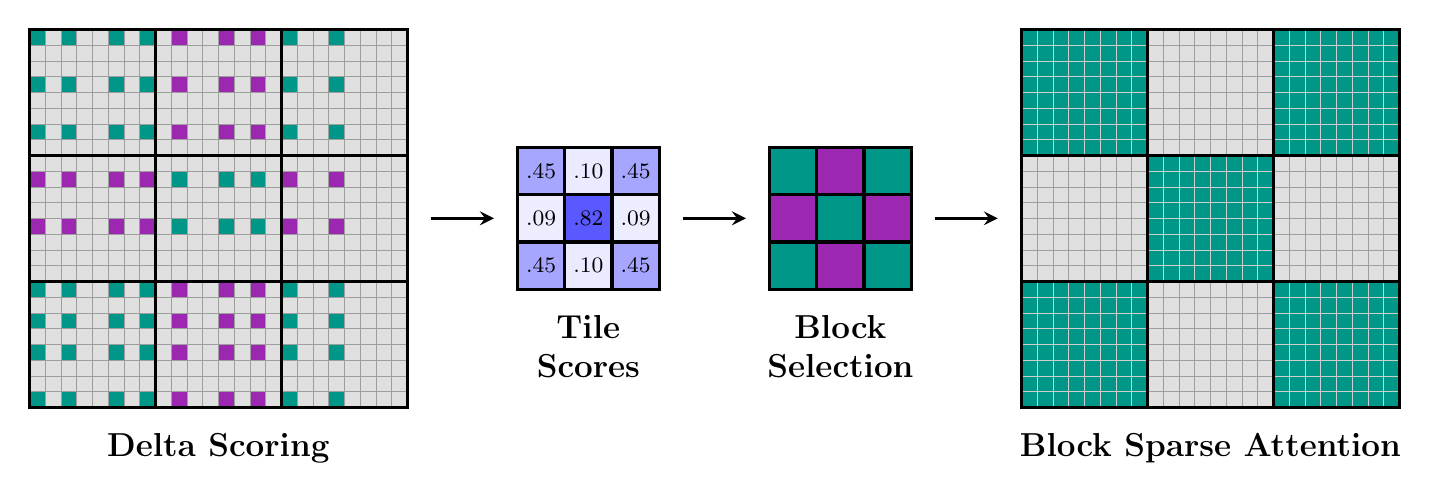
\begin{tikzpicture}[>=stealth, thick]

  % Colors
  \definecolor{selcolor}{HTML}{009688} % Teal
  \definecolor{unselcolor}{HTML}{9C27B0} % Purple
  \definecolor{bglight}{HTML}{E0E0E0}
  \definecolor{gridcolor}{HTML}{9E9E9E}

  \def\cell{0.2} % cell size for left and right
  \def\bcell{1.6} % big cell size = 8 * 0.2
  \def\mcell{0.6} % small (3x3) grid cell size

  % PART 1: Delta Scoring
  \begin{scope}[shift={(0,0)}]
    % Draw background and small grid
    \fill[bglight] (0,0) rectangle (3*\bcell, -3*\bcell);
    \draw[gridcolor, very thin, step=\cell] (0,0) grid (3*\bcell, -3*\bcell);

    % Draw grid-sampled cells: intersection of Q-anchor rows and K-anchor cols
    \foreach \br in {0,1,2} {
      \foreach \bc in {0,1,2} {
        % Determine if block is selected: X pattern => br == bc or br+bc == 2
        \pgfmathtruncatemacro{\issel}{(\br==\bc) || (\br+\bc==2)}
        \ifnum\issel=1
          \colorlet{dcolor}{selcolor}
        \else
          \colorlet{dcolor}{unselcolor}
        \fi

        \foreach \r in {0,...,7} {
          \foreach \c in {0,...,7} {
            % Q anchors depend on the block-row, K anchors on the block-column,
            % so each tile gets its own content-adaptive grid.
            \pgfmathtruncatemacro{\isrow}{
              ((\br==0) && ((\r==0)||(\r==3)||(\r==6))) ||
              ((\br==1) && ((\r==1)||(\r==4))) ||
              ((\br==2) && ((\r==0)||(\r==2)||(\r==4)||(\r==7)))
            }
            \pgfmathtruncatemacro{\iscol}{
              ((\bc==0) && ((\c==0)||(\c==2)||(\c==5)||(\c==7))) ||
              ((\bc==1) && ((\c==1)||(\c==4)||(\c==6))) ||
              ((\bc==2) && ((\c==0)||(\c==3)))
            }
            \pgfmathtruncatemacro{\isgrid}{\isrow && \iscol}
            \ifnum\isgrid=1
              \fill[dcolor] ({\bc*\bcell + \c*\cell}, {-\br*\bcell - \r*\cell}) rectangle ++(\cell, -\cell);
              \draw[gridcolor, very thin] ({\bc*\bcell + \c*\cell}, {-\br*\bcell - \r*\cell}) rectangle ++(\cell, -\cell);
            \fi
          }
        }
      }
    }
    % Draw thick big block borders
    \draw[very thick, step=\bcell] (0,0) grid (3*\bcell, -3*\bcell);
    \draw[very thick] (0,0) rectangle (3*\bcell, -3*\bcell);
    \node[below, font=\large\bfseries] at (1.5*\bcell, -3*\bcell - 0.2) {Delta Scoring};
  \end{scope}

  % Arrow 1
  \draw[->, very thick] (3*\bcell + 0.3, -1.5*\bcell) -- ++(0.8, 0);

  % PART 2: Tile Scores (weight per tile, normalized per query row)
  \begin{scope}[shift={(3*\bcell + 1.4, -1.5*\bcell + 1.5*\mcell)}]
    \foreach \br/\bc/\val/\xf in {
      0/0/.45/35, 0/1/.10/8,  0/2/.45/35,
      1/0/.09/7,  1/1/.82/65, 1/2/.09/7,
      2/0/.45/35, 2/1/.10/8,  2/2/.45/35}
    {
      \fill[blue!\xf] (\bc*\mcell, -\br*\mcell) rectangle ++(\mcell, -\mcell);
      \draw[very thick] (\bc*\mcell, -\br*\mcell) rectangle ++(\mcell, -\mcell);
      \node[font=\footnotesize] at ({(\bc+0.5)*\mcell}, {-(\br+0.5)*\mcell}) {\val};
    }
    \draw[very thick] (0,0) rectangle (3*\mcell, -3*\mcell);
    \node[below, align=center, font=\large\bfseries] at (1.5*\mcell, -3*\mcell - 0.2) {Tile\\Scores};
  \end{scope}

  % Arrow 2
  \draw[->, very thick] (3*\bcell + 1.4 + 3*\mcell + 0.3, -1.5*\bcell) -- ++(0.8, 0);

  % PART 3: Block Selection
  \begin{scope}[shift={(3*\bcell + 1.4 + 3*\mcell + 1.4, -1.5*\bcell + 1.5*\mcell)}]
    \foreach \br in {0,1,2} {
      \foreach \bc in {0,1,2} {
        \pgfmathtruncatemacro{\issel}{(\br==\bc) || (\br+\bc==2)}
        \ifnum\issel=1
          \fill[selcolor] (\bc*\mcell, -\br*\mcell) rectangle ++(\mcell, -\mcell);
        \else
          \fill[unselcolor] (\bc*\mcell, -\br*\mcell) rectangle ++(\mcell, -\mcell);
        \fi
        \draw[very thick] (\bc*\mcell, -\br*\mcell) rectangle ++(\mcell, -\mcell);
      }
    }
    \draw[very thick] (0,0) rectangle (3*\mcell, -3*\mcell);
    \node[below, align=center, font=\large\bfseries] at (1.5*\mcell, -3*\mcell - 0.2) {Block\\Selection};
  \end{scope}

  % Arrow 3
  \draw[->, very thick] (3*\bcell + 1.4 + 3*\mcell + 1.4 + 3*\mcell + 0.3, -1.5*\bcell) -- ++(0.8, 0);

  % PART 4: Block Sparse Attention
  \begin{scope}[shift={(3*\bcell + 1.4 + 3*\mcell + 1.4 + 3*\mcell + 1.4, 0)}]
    \fill[bglight] (0,0) rectangle (3*\bcell, -3*\bcell);
    \draw[gridcolor, very thin, step=\cell] (0,0) grid (3*\bcell, -3*\bcell);

    \foreach \br in {0,1,2} {
      \foreach \bc in {0,1,2} {
        \pgfmathtruncatemacro{\issel}{(\br==\bc) || (\br+\bc==2)}
        \ifnum\issel=1
          \fill[selcolor] (\bc*\bcell, -\br*\bcell) rectangle ++(\bcell, -\bcell);
          % We can re-draw the small grid over it if we want it to look like the original
          \draw[gridcolor!50!white, very thin, step=\cell, shift={(\bc*\bcell, -\br*\bcell)}] (0,0) grid (\bcell, -\bcell);
        \fi
      }
    }

    \draw[very thick, step=\bcell] (0,0) grid (3*\bcell, -3*\bcell);
    \draw[very thick] (0,0) rectangle (3*\bcell, -3*\bcell);
    \node[below, font=\large\bfseries] at (1.5*\bcell, -3*\bcell - 0.2) {Block Sparse Attention};
  \end{scope}

\end{tikzpicture}
}
\caption{DPXA four-stage process: Delta scoring samples, within each tile, the cells where a $Q$ anchor row meets a $K$ anchor column; anchors are selected per block, so the content-adaptive grid differs from tile to tile. Exponentiating and summing a tile's sampled scores gives its weight, normalized across each query row. Block selection keeps the top-scoring tiles per row (teal) and drops the rest (purple). Block sparse attention computes the full attention only for the selected blocks.}
\label{fig:dpxa_3part}
\end{figure}
%% ---- end diagrams/dpxa_3part ----

% ==================== experimental_setup ====================
\section{Experimental Setup}

\subsection{Benchmarks}

\subsubsection{Needle in a Haystack and RULER}

Benchmarks for long-context transformers are a big research area by themselves. The original Needle in a Haystack (NIAH) test inserts a distinctive sentence at a random position in a long text and asks the model to retrieve it. NIAH only tests retrieval and is a limited evaluation method on its own. Models that do well on NIAH can still fail on real-world tasks~\cite{kuratov2024babilong}.

RULER~\cite{hsieh2024ruler} is the modern extension of NIAH, expanding it to 13 tasks such as multi-hop variable tracking and question answering over long contexts. RULER has become a standard benchmark in the field, with MInference~\cite{jiang2024minference}, FlexPrefill~\cite{lai2025flexprefill}, and XAttention~\cite{xu2025xattention} all reporting results on it. RULER evaluates models at a range of context lengths, typically from 4K to 128K tokens. DeltaAttention is evaluated on RULER for a direct comparison with existing methods.

\textbf{Our RULER setup.} The standard RULER setup uses 100 samples per task across all 13 tasks, which is very expensive to run. We therefore utilize two setups. The light setup uses 30 samples per task across 9 tasks (niah\_single\_1/2/3, niah\_multikey\_1/2/3, vt, cwe, fwe), it drops the question-answering tasks from the full set, as these are real-world style tasks already covered by LongBench. The full setup uses the standard 100 samples per task across all 13 tasks.

We use the light setup during development and for the results and ablations of Delta-KV compression, DeltaXAttention, and the DPXA ablations. It is cheap enough to run repeatedly across many configurations, and the synthetic retrieval tasks give a sensitive signal on attention health. The full setup is reserved for our main DPXA results, where we report against the strongest baselines and want a complete picture.

\subsubsection{LongBench}

LongBench~\cite{bai2024longbench} is another standard benchmark used in the field. Unlike RULER, which uses synthetic tasks, LongBench uses real-world documents from tasks such as coding, question answering, and summarization, at context lengths from roughly 3K to 24K tokens. It covers 21 datasets across six task categories: single-document QA, multi-document QA, summarization, few-shot learning, synthetic retrieval, and code completion. We use 100 samples per task. For our main DPXA results we evaluate on 16 of these tasks, and for the DPXA cosine threshold sweep we use a reduced set of 9 tasks spanning single-document QA, multi-document QA, and summarization. As with RULER, only DPXA is reported on LongBench, since it is our most promising method. LongBench is a good complement to RULER because it uses real documents rather than synthetic retrieval.

\subsubsection{Video-MME}

RULER and LongBench are both text benchmarks. To test whether DPXA also works on video, we evaluate on Video-MME~\cite{fu2024videomme}, a long video understanding benchmark. The task is multiple-choice question answering over videos. We evaluate on Qwen2-VL-7B-Instruct, sampling each video at 1 frame per second. The benchmark uses 2,700 videos with durations ranging from short (under 2 minutes) to long (30 to 60 minutes), which lets us see how DPXA behaves as the context gets longer. As with the full RULER and LongBench setups, only DPXA is reported on Video-MME. Our main results use the full 2,700-video test set, while the packing threshold ablations use a reduced 200-video subset, since the ablations sweep many configurations.

\subsection{Speedup Experiment}

To measure raw attention speedup, we run an isolated prefill test independent of any downstream task, following the latency evaluation in MInference~\cite{jiang2024minference}. The model is fed a randomly sampled sequence from WikiText-103 across a range of context lengths. We measure the time to first token, which covers the full prefill stage. DeltaAttention is compared against PyTorch SDPA, which dispatches to a FlashAttention-2 kernel, as the dense baseline. For each method and context length we discard 2 warmup iterations, so that measurements reflect steady-state kernel performance, and then report the mean prefill latency over 10 timed runs. Latency is measured with CUDA events synchronized around the forward pass.

% ==================== results ====================
\section{Results}

We report results for the three methods in turn: Delta-KV compression, DeltaXAttention, and delta-based tile scoring (DPXA). All evaluations use LLaMA-3.1 8B Instruct. Delta-KV compression and DeltaXAttention are evaluated exclusively on RULER, while DPXA is evaluated on both RULER and LongBench. We chose this strategy because synthetic retrieval tasks (such as those in RULER) provide a sensitive measure of attention pattern fidelity, making them well-suited for rapid evaluation during development. Additionally, because Delta-KV and DeltaXAttention are less competitive with current state-of-the-art approaches, we limit their evaluation to RULER and reserve the LongBench suite for our most promising method, DPXA.

\subsection{Delta-KV Compression}

\subsubsection{RULER}

Table~\ref{tab:ruler} reports RULER accuracy on LLaMA-3.1 8B Instruct across context lengths from 4K to 128K tokens. All methods are run from their respective codebases. Looking at the average scores, Delta-KV performs similarly to MInference, and both are slightly below XAttention, but the gap is small. Both XAttention and Delta-KV degrade at 64K tokens, while MInference retains accuracy at that length. Conversely, at 128K tokens, MInference degrades significantly, whereas Delta-KV and XAttention retain good accuracy. However, drawing strong conclusions from these two observations would be inaccurate, as this relies on a reduced RULER setup. Overall, Delta-KV achieves comparable accuracy to state-of-the-art methods while reducing KV loads by 50.9\%.

\begin{table}[!ht]
\centering
\caption{RULER accuracy (\%) on LLaMA-3.1 8B Instruct (30 samples, 9 tasks). Higher is better. KV Red is the average fraction of KV loads saved relative to full attention.}
\label{tab:ruler}
\begin{tabular}{lrrrrrrrr}
\toprule
Method & 4K & 8K & 16K & 32K & 64K & 128K & Avg & KV Red \\
\midrule
Full attention            & 99.31 & 97.21 & 96.59 & 93.76 & 88.23 & 74.00 & 91.52 & 0\%    \\
MInference                & 99.18 & 97.25 & 96.44 & 91.96 & 87.21 & 65.26 & 89.55 & --     \\
XAttention                & 98.14 & 97.37 & 96.62 & 92.84 & 84.01 & 71.49 & 90.08 & --     \\
Delta-KV (cos\,0.83)         & 99.27 & 96.99 & 95.11 & 90.79 & 83.94 & 71.43 & 89.59 & 50.9\% \\
\bottomrule
\end{tabular}
\end{table}

\subsubsection{Speedup analysis}

Figure~\ref{fig:speedup_comparison} shows the prefill speedup of Delta-KV at cos\,0.83 and cos\,0.78 against two baselines.
The Flash baseline is our own Triton FlashAttention-2 implementation, which is the same kernel Delta-KV is built on, so this is a direct comparison of the effect of delta packing alone.
SDPA is a standard PyTorch FlashAttention-2 implementation included as a common reference point.

At short sequences the overhead of computing the delta pattern costs more than it saves, so Delta-KV is slower.
Around 16K tokens the reduction in K iterations starts to dominate and Delta-KV crosses above both baselines.
At 262K tokens, cos\,0.83 reaches roughly 1.35x over SDPA and 1.5x over Flash, while cos\,0.78 reaches roughly 1.8x over SDPA and 2.1x over Flash.

The observed speedup is lower than what the KV reduction alone would predict.
cos\,0.83 achieves 50\% KV reduction (Section~\ref{sec:ablation_threshold}), which would suggest a 2x attention speedup, but attention is only one part of the forward pass: MLP layers take a fixed share of the time regardless of sequence length.
As sequence length grows, attention increasingly dominates latency (Figure~\ref{fig:attention_dominance}), so the end-to-end speedup approaches the theoretical attention speedup.
Our experiments on an H100 ran up to 262K tokens, and the trend suggests the speedup would continue climbing toward 2x.
At cos\,0.78, the 65\% KV reduction implies a theoretical attention speedup of roughly 3x, but the measured value is 2.1x at 262K for the same reason.

A second factor limiting the realized speedup is the overhead of delta computation and packing (Sections~\ref{sec:preprocessing} and~\ref{sec:packing}).
Figure~\ref{fig:delta_overhead} shows that at 512 tokens this overhead accounts for 39.1\% of total prefill time, dropping to 22.6\% at 4K and 8.5\% at 16K.
The overhead grows slowly with sequence length, from 21ms at 512 tokens to 95ms at 262K, while the total prefill time grows much faster.
As a result the ratio falls to 1.4\% at 65K tokens and 0.24\% at 262K, making it negligible at the sequence lengths where Delta-KV provides the most speedup.

A final factor is that the Delta-KV kernel cannot benefit from memory pipelining.
Standard FlashAttention iterates over key blocks with a for loop, so the GPU can prefetch the next block's data from HBM while the current block's matrix multiply is still running, hiding most of the memory latency.
Delta-KV uses a while loop to handle the two phases dynamically, and the number of iterations is not known in advance, so the compiler cannot schedule prefetches ahead of time.
Each block load must complete before the next iteration can start.
This is an inherent cost of the adaptive two-phase structure and one of the main reasons Delta-KV does not fully realize its theoretical speedup.




\begin{figure}[!ht]
    \centering
    
\includegraphics[width=\linewidth]{assets/speedup_comparison.png}
    \caption{Prefill speedup of Delta-KV relative to SDPA and Flash baselines at cos\,0.83 (left) and cos\,0.78 (right) on LLaMA-3.1 8B Instruct. Values above 1.0 mean Delta-KV is faster.}
    \label{fig:speedup_comparison}
\end{figure}

\begin{figure}[!ht]
\centering
\begin{subfigure}[b]{0.48\textwidth}
    \centering
    
\includegraphics[width=\linewidth]{assets/attention_dominance.png}
    \caption{Attention compute as a fraction of total prefill time.}
    \label{fig:attention_dominance}
\end{subfigure}
\hfill
\begin{subfigure}[b]{0.48\textwidth}
    \centering
    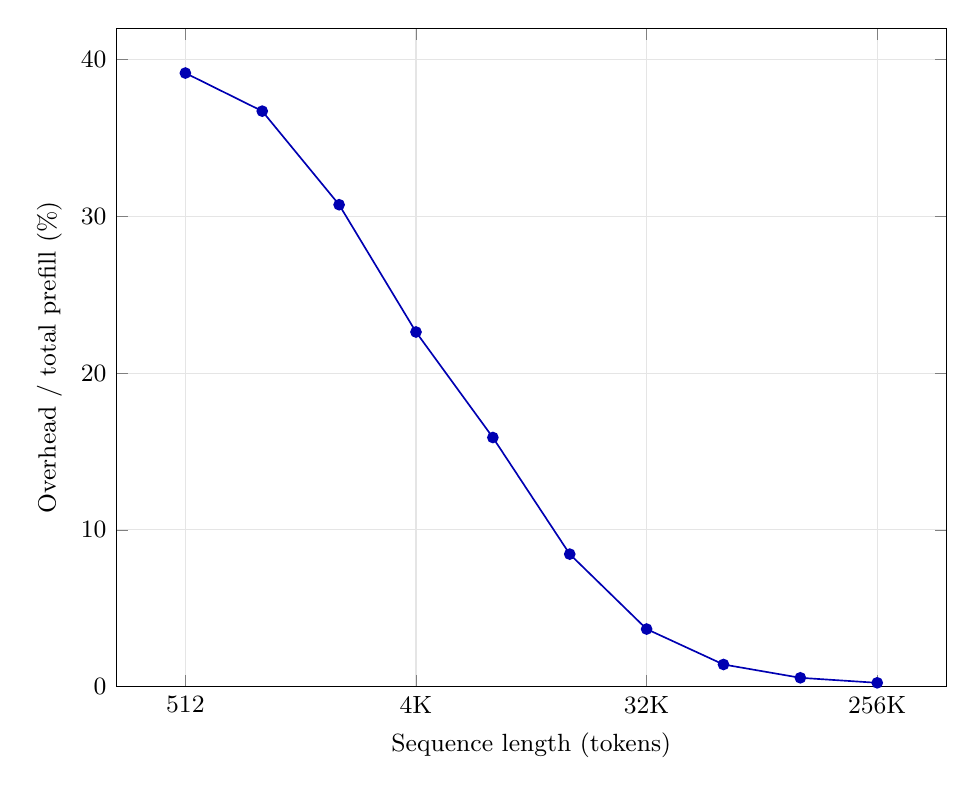
\begin{tikzpicture}
    \begin{axis}[
        width=\linewidth, height=0.82\linewidth,
        xmode=log, log basis x=2,
        xtick={512,4096,32768,262144},
        xticklabels={512,4K,32K,256K},
        xlabel={Sequence length (tokens)},
        ylabel={Overhead / total prefill (\%)},
        ymin=0, ymax=42,
        ytick={0,10,20,30,40},
        grid=both, grid style={gray!20},
        tick label style={font=\small},
        label style={font=\small},
        mark size=1.8pt,
    ]
    \addplot[color=blue!70!black, semithick, mark=*]
        coordinates {(512,39.14)(1024,36.71)(2048,30.74)(4096,22.62)(8192,15.89)(16384,8.45)(32768,3.67)(65536,1.41)(131072,0.56)(262144,0.24)};
    \end{axis}
    \end{tikzpicture}
    \caption{Delta computation and packing overhead as a fraction of total prefill time.}
    \label{fig:delta_overhead}
\end{subfigure}
\caption{Prefill time breakdown for Delta-KV at cos\,0.83 on LLaMA-3.1 8B Instruct, across sequence length. (a) Attention grows to dominate the forward pass, from a small fraction at short sequences to 95\% at 262K tokens. (b) The delta computation and packing overhead shrinks from 39\% of prefill at 512 tokens to 0.24\% at 262K, becoming negligible at the lengths where Delta-KV provides the most speedup.}
\label{fig:prefill_breakdown}
\end{figure}



\subsubsection{Ablations}

In this section we ablate the threshold metric and the main design choices of Delta-KV compression.

\paragraph{Threshold metric.}
\label{sec:ablation_threshold}

Table~\ref{tab:ablation_threshold} compares Euclidean distance and cosine similarity as the threshold metric in the pre-processing stage. Pairs of rows are matched by KV reduction level: low (~30\%), medium (~50\%), and high (~65\%). Both metrics perform similarly at low compression, but cosine is consistently better at higher compression, most visibly at 128K tokens where it retains 66.57\% accuracy versus 60.57\% for Euclidean at 65\% KV reduction. Cosine is the better metric overall. We use cos\,0.83 (50\% KV reduction) as the default operating point: it roughly halves the KV loads with minimal accuracy loss, whereas the 30\% setting yields too little speedup and the 65\% setting loses more accuracy. The subsequent ablation studies in this section use Euclidean thresholds; however, because the two metrics behave very similarly, all insights derived from Euclidean thresholding are valid.

\begin{table}[!ht]
\centering
\caption{RULER accuracy (\%) comparing Euclidean and cosine thresholds (30 samples, 9 tasks). Pairs are matched by KV reduction.}
\label{tab:ablation_threshold}
\begin{tabular}{lrrrrrrrr}
\toprule
Method & 4K & 8K & 16K & 32K & 64K & 128K & Avg & KV Red \\
\midrule
Full attention              & 99.31 & 97.41 & 96.52 & 93.65 & 88.16 & 74.35 & 91.57 & 0\%    \\
\midrule
Euclidean t13               & 99.11 & 96.63 & 95.63 & 92.31 & 86.96 & 75.19 & 90.97 & 32.0\% \\
Cosine cos\,0.88               & 99.38 & 97.54 & 96.70 & 92.31 & 86.73 & 72.82 & 90.91 & 29.5\% \\
\midrule
Euclidean t15               & 97.94 & 96.05 & 94.04 & 91.62 & 83.77 & 69.44 & 88.81 & 49.7\% \\
Cosine cos\,0.83               & 99.27 & 96.99 & 95.11 & 90.79 & 83.94 & 71.43 & 89.59 & 50.9\% \\
\midrule
Euclidean t17               & 98.27 & 96.27 & 93.36 & 90.45 & 82.16 & 60.57 & 86.85 & 65.2\% \\
Cosine cos\,0.78               & 99.01 & 97.12 & 94.07 & 86.99 & 81.27 & 66.57 & 87.50 & 65.8\% \\
\bottomrule
\end{tabular}
\end{table}

\paragraph{Count-weighted softmax.}

Count-weighted softmax is theoretically necessary for correctness: without it, an anchor representing many tokens receives the same attention weight as one representing a single token, which underestimates its contribution. With it, the result is equivalent to exact attention where each anchor key is repeated for every token it covers (Section~\ref{sec:self_attention_compressed}).

Table~\ref{tab:ablation_count} shows that removing count-weighted softmax has almost no effect on accuracy across all three compression levels. If anything, dropping it is slightly better: it wins at two of the three levels and is a touch higher on average (89.12 versus 88.88). A likely explanation is that the per-anchor counts are similar across anchors in practice, so the scaling barely shifts the softmax distribution, and the small differences are within noise.

So count-weighting keeps the method theoretically correct but does not help accuracy in practice. We keep it on for the Delta-KV results in this section, since it preserves the exact-attention equivalence at no real cost. For the two methods that follow, DeltaXAttention and DPXA, we disable count-weighting: it does not improve accuracy, and turning it off keeps those methods simpler. This is why the count-weighting is off in all later experiments and not mentioned.

\begin{table}[!ht]
\centering
\caption{RULER accuracy (\%) with and without count-weighted softmax (30 samples, 9 tasks).}
\label{tab:ablation_count}
\begin{tabular}{lrrrrrrrr}
\toprule
Method & 4K & 8K & 16K & 32K & 64K & 128K & Avg & KV Red \\
\midrule
Full attention                 & 99.31 & 97.41 & 96.52 & 93.65 & 88.16 & 74.35 & 91.57 & 0\%    \\
\midrule
Delta-KV t13             & 99.11 & 96.63 & 95.63 & 92.31 & 86.96 & 75.19 & 90.97 & 32.0\% \\
Delta-KV t15             & 97.94 & 96.05 & 94.04 & 91.62 & 83.77 & 69.44 & 88.81 & 49.7\% \\
Delta-KV t17             & 98.27 & 96.27 & 93.36 & 90.45 & 82.16 & 60.57 & 86.85 & 65.2\% \\
\midrule
w/o count-weighted softmax t13 & 98.90 & 97.31 & 95.32 & 94.25 & 86.62 & 75.31 & 91.29 & 30.9\% \\
w/o count-weighted softmax t15 & 98.68 & 95.52 & 95.00 & 91.43 & 81.55 & 69.74 & 88.65 & 48.8\% \\
w/o count-weighted softmax t17 & 98.62 & 96.05 & 94.04 & 89.72 & 79.00 & 67.04 & 87.41 & 64.7\% \\
\bottomrule
\end{tabular}
\end{table}

\paragraph{Critical diagonal.}

The diagonal band of the attention matrix carries the majority of attention mass, as each token attends most strongly to its immediate neighbors (Section~\ref{sec:local_attention_window}). Phase 2 of the Delta-KV kernel switches to exact uncompressed attention for the tiles covering this band, so those neighbor interactions are computed precisely (Section~\ref{sec:flash_attention_adaptation}).

Table~\ref{tab:ablation_diag} shows that removing phase 2 causes a catastrophic accuracy drop across all compression levels. At t13 the average falls from 90.97\% to 57.90\%, and at t17 it collapses to 15.19\%. Phase 2 is a critical component of Delta-KV.

\begin{table}[!ht]
\centering
\caption{RULER accuracy (\%) with and without phase 2 (critical diagonal) (30 samples, 9 tasks).}
\label{tab:ablation_diag}
\begin{tabular}{lrrrrrrrr}
\toprule
Method & 4K & 8K & 16K & 32K & 64K & 128K & Avg & KV Red \\
\midrule
Full attention                    & 99.31 & 97.41 & 96.52 & 93.65 & 88.16 & 74.35 & 91.57 & 0\%    \\
\midrule
Delta-KV t13                & 99.11 & 96.63 & 95.63 & 92.31 & 86.96 & 75.19 & 90.97 & 32.0\% \\
Delta-KV t15                & 97.94 & 96.05 & 94.04 & 91.62 & 83.77 & 69.44 & 88.81 & 49.7\% \\
Delta-KV t17                & 98.27 & 96.27 & 93.36 & 90.45 & 82.16 & 60.57 & 86.85 & 65.2\% \\
\midrule
w/o phase 2 (critical diag.) t13  & 74.16 & 64.04 & 61.70 & 58.39 & 50.36 & 38.75 & 57.90 & 35.7\% \\
w/o phase 2 (critical diag.) t15  & 54.75 & 45.15 & 42.72 & 37.41 & 35.44 & 19.85 & 39.22 & 55.0\% \\
w/o phase 2 (critical diag.) t17  & 17.19 & 18.44 & 19.82 & 17.07 & 11.85 &  6.79 & 15.19 & 71.3\% \\
\bottomrule
\end{tabular}
\end{table}

\paragraph{Phase 2 only.}

In this ablation all phase 1 iterations are skipped. Only the diagonal band tiles are computed exactly. Tokens attend only to their immediate neighbors and have no access to the compressed history from phase 1. Table~\ref{tab:ablation_phase2only} shows accuracy collapse, confirming that the compressed history carried by phase 1 is essential.

The small accuracy increase from t13 to t17 is an artifact of how the critical diagonal is determined. Phase 2 starts as soon as a packed key block's reach overlaps with the current query block's span. At higher thresholds each anchor represents a longer range, so packed blocks reach further into the sequence and the critical diagonal is entered earlier. This means phase 2 computes more exact tiles near the diagonal at higher thresholds, giving a slight accuracy boost. This is a useful property of the algorithm: higher compression thresholds naturally expand the exact local window, partially compensating for the coarser compressed history.

\begin{table}[!ht]
\centering
\caption{RULER accuracy (\%) for phase 2 only (local diagonal, no compressed history) (30 samples, 9 tasks).}
\label{tab:ablation_phase2only}
\begin{tabular}{lrrrrrrrr}
\toprule
Method & 4K & 8K & 16K & 32K & 64K & 128K & Avg & KV Red \\
\midrule
Full attention                   & 99.31 & 97.41 & 96.52 & 93.65 & 88.16 & 74.35 & 91.57 & 0\%    \\
\midrule
Delta-KV t13               & 99.11 & 96.63 & 95.63 & 92.31 & 86.96 & 75.19 & 90.97 & 32.0\% \\
Delta-KV t15               & 97.94 & 96.05 & 94.04 & 91.62 & 83.77 & 69.44 & 88.81 & 49.7\% \\
Delta-KV t17               & 98.27 & 96.27 & 93.36 & 90.45 & 82.16 & 60.57 & 86.85 & 65.2\% \\
\midrule
phase 2 only t13                 & 12.97 & 11.01 &  6.62 &  3.32 &  3.53 &  1.98 &  6.57 & 40.2\% \\
phase 2 only t15                 & 14.17 & 10.62 &  8.59 &  4.63 &  3.86 &  1.85 &  7.29 & 56.0\% \\
phase 2 only t17                 & 17.27 & 10.44 &  8.84 &  5.10 &  3.78 &  2.10 &  7.92 & 67.9\% \\
\bottomrule
\end{tabular}
\end{table}

\paragraph{Non-adaptive baselines.}

The phase 2 only ablation showed that the compressed history is essential for retrieval. Here we check whether Delta-KV's content-adaptive key selection is what makes it effective, or whether any compression scheme at the same reduction works. Random packing randomly drops key vectors to reach a target compression. Periodic packing keeps every $n$th token and drops the rest, with $n=2$ giving 50\% reduction and $n=3$ giving 65\% reduction. These match the KV reductions of Delta-KV t15 and t17 for direct comparison.

Both baselines retain some performance, but Delta-KV is consistently better. At 50\% reduction, periodic packing is surprisingly competitive at 87.46\% versus 88.81\% for Delta-KV, while random packing falls to 84.22\%. At 65\% reduction the gap widens: Delta-KV holds at 86.85\%, periodic drops to 81.85\%, and random to 75.12\%. The content-adaptive selection becomes more important at higher compression.

\begin{table}[!ht]
\centering
\caption{RULER accuracy (\%) comparing Delta-KV against non-adaptive packing baselines at matched KV reduction (30 samples, 9 tasks).}
\label{tab:ablation_packing}
\begin{tabular}{lrrrrrrrr}
\toprule
Method & 4K & 8K & 16K & 32K & 64K & 128K & Avg & KV Red \\
\midrule
Full attention              & 99.31 & 97.41 & 96.52 & 93.65 & 88.16 & 74.35 & 91.57 & 0\%    \\
\midrule
Delta-KV t15          & 97.94 & 96.05 & 94.04 & 91.62 & 83.77 & 69.44 & 88.81 & 49.7\% \\
periodic packing (kr=50\%)  & 97.53 & 95.01 & 92.80 & 90.90 & 81.62 & 66.91 & 87.46 & 50.0\% \\
random packing (kr=50\%)    & 97.17 & 92.51 & 91.22 & 83.83 & 75.72 & 64.88 & 84.22 & 50.0\% \\
\midrule
Delta-KV t17          & 98.27 & 96.27 & 93.36 & 90.45 & 82.16 & 60.57 & 86.85 & 65.2\% \\
periodic packing (kr=35\%)  & 92.12 & 91.02 & 86.57 & 83.19 & 75.15 & 63.06 & 81.85 & 66.7\% \\
random packing (kr=35\%)    & 89.62 & 86.61 & 80.26 & 73.81 & 68.08 & 52.37 & 75.12 & 65.0\% \\
\bottomrule
\end{tabular}
\end{table}

\subsection{DeltaXAttention}

Table~\ref{tab:deltaxattn} evaluates DeltaXAttention as described in Section~\ref{sec:xattention_adaptation}. We introduce three variants of DeltaXAttention: packing all selected tiles (all packed), computing diagonal tiles exactly (diag kept), and computing both the diagonal and the top 10\% most important off-diagonal tiles exactly (tw10). As a baseline comparison, we increase XAttention's sparsity by dropping its least important 40\%, 50\%, and 60\% of tiles (XAttn tile skip dr=40\%, 50\%, 60\%). This tile skipping provides a matched KV reduction to our DeltaXAttention variants at compression thresholds dt=13, 15, and 17, respectively, allowing us to compare accuracy retention at fixed KV reduction levels.

Applying delta packing to all tiles XAttention selects (DeltaXAttn all packed) results in severe accuracy degradation: 51.39\% at dt=13 and 12.81\% at dt=17. This mirrors the critical diagonal finding in Section~\ref{sec:flash_attention_adaptation}: packing the diagonal tiles only approximates the neighbor interactions that carry the most attention mass. Computing diagonal tiles exactly (DeltaXAttn diag kept) recovers accuracy dramatically.

Adding a second accuracy guard, computing the top 10\% of off-diagonal tiles exactly as well (DeltaXAttn tw10), recovers additional accuracy. At dt=15, this configuration achieves 87.06\% with 45.6\% KV reduction relative to XAttention, a loss of 3.0 percentage points against the XAttention baseline.

The key question is whether XAttention could have achieved the same KV reduction natively by skipping more tiles. At matched reductions, DeltaXAttn tw10 consistently outperforms XAttention tile skipping by a small margin: 88.95\% vs 87.51\% at ~37\% reduction, 87.06\% vs 85.98\% at ~46\%, and 85.14\% vs 84.43\% at ~57\%. However, skipped tiles in XAttention translate directly to fewer FlashAttention iterations, which is straightforward to realize as speedup. DeltaXAttention saves KV loads within each iteration, which is harder to exploit in practice since it does not reduce the number of tiles processed. We conclude that DeltaXAttention can further optimize block-sparse attention methods with minimal accuracy degradation, but its practical value here is limited: XAttention can achieve similar reductions through tile skipping with comparable accuracy and a more direct path to speedup.



\begin{table}[!ht]
\centering
\caption{RULER accuracy (\%) for DeltaXAttention ablation on LLaMA-3.1 8B Instruct (30 samples, 9 tasks). KV Red is relative to standard XAttention.}
\label{tab:deltaxattn}
\begin{tabular}{lrrrrrrrr}
\toprule
Method & 4K & 8K & 16K & 32K & 64K & 128K & Avg & KV Red \\
\midrule
XAttention                    & 98.14 & 97.37 & 96.62 & 92.84 & 84.01 & 71.49 & 90.08 & 0\%    \\
\midrule
XAttn tile skip dr=40\%       & 98.47 & 95.56 & 92.63 & 89.51 & 81.26 & 67.64 & 87.51 & 37.4\% \\
XAttn tile skip dr=50\%       & 98.72 & 94.20 & 91.05 & 89.43 & 78.67 & 63.81 & 85.98 & 48.4\% \\
XAttn tile skip dr=60\%       & 97.48 & 93.86 & 89.53 & 88.05 & 76.83 & 60.83 & 84.43 & 57.6\% \\
\midrule
DeltaXAttn all packed dt=13   & 68.00 & 62.83 & 59.12 & 53.72 & 42.00 & 22.69 & 51.39 & 38.8\% \\
DeltaXAttn all packed dt=15   & 55.53 & 48.63 & 40.59 & 33.95 & 28.27 & 23.86 & 38.47 & 54.8\% \\
DeltaXAttn all packed dt=17   & 19.17 & 17.14 & 15.06 & 12.01 & 10.04 &  3.46 & 12.81 & 70.1\% \\
\midrule
DeltaXAttn diag kept dt=13    & 97.64 & 95.68 & 94.01 & 91.75 & 77.75 & 67.61 & 87.41 & 36.2\% \\
DeltaXAttn diag kept dt=15    & 96.24 & 93.38 & 92.15 & 88.63 & 75.74 & 61.95 & 84.68 & 50.5\% \\
DeltaXAttn diag kept dt=17    & 95.06 & 93.46 & 90.65 & 84.47 & 65.72 & 51.53 & 80.15 & 63.5\% \\
\midrule
DeltaXAttn tw10 dt=13         & 97.90 & 96.36 & 95.21 & 91.73 & 82.62 & 69.90 & 88.95 & 32.3\% \\
DeltaXAttn tw10 dt=15         & 97.99 & 95.04 & 94.22 & 89.57 & 80.27 & 65.28 & 87.06 & 45.6\% \\
DeltaXAttn tw10 dt=17         & 97.54 & 95.19 & 92.48 & 87.15 & 75.62 & 62.89 & 85.14 & 57.0\% \\
\bottomrule
\end{tabular}
\end{table}

\subsection{Delta-Based Tile Scoring (DPXA)}
\label{sec:results_delta_tile_scoring}

We evaluate delta-based tile scoring (DPXA) against a set of strong training-free sparse attention baselines. DPXA is the direct descendant of XAttention, so XAttention at stride 8 and stride 16, at recall $r{=}0.90$, are the most direct comparison points. We also compare against MInference and FlexPrefill, which together cover the main lines of work in training-free sparse attention. We exclude SpargeAttention from our comparisons, as its implementation is bundled with quantization; this introduces latency reductions unrelated to sparse attention, making a clean comparison with the rest of the methods impossible. All baselines are run from their original GitHub repositories, with no reimplementation. We report DPXA at two cosine thresholds, $0.72$ and $0.78$, both at recall $r{=}0.90$. Unlike the earlier sections, we evaluate DPXA on the full RULER (100 samples, 13 tasks) and full LongBench (16 tasks), together with an isolated speedup analysis from 4K to 512K.


\subsubsection{RULER}

Table~\ref{tab:delta_tile_scoring} reports RULER accuracy. DPXA is close to lossless: cos\,0.72 scores 88.97 and cos\,0.78 scores 89.02, both within 0.1 points of full attention (89.07). Both settings beat every sparse baseline we test. The closest comparison is XAttention, which DPXA outscores on average (88.02 at stride 16, 87.70 at stride 8). The gap is largest at 128K tokens, where DPXA holds 75.55 (cos\,0.78) and 74.82 (cos\,0.72), while XAttention falls to 70.96 (stride 16) and 71.57 (stride 8). DPXA also beats MInference (86.57) and FlexPrefill (87.45) on average.

\begin{table}[!ht]
\centering
\caption{RULER accuracy (\%) comparing delta-based tile scoring against baseline and block-sparse methods on LLaMA-3.1 8B Instruct (100 samples, 13 tasks). DPXA and FlexPrefill are both at recall/coverage target $0.90$ ($r{=}0.90$ and $\gamma{=}0.90$ respectively). Best score per column in \textbf{bold}.}
\label{tab:delta_tile_scoring}
\begin{tabular}{lrrrrrrr}
\toprule
Method & 4K & 8K & 16K & 32K & 64K & 128K & Avg \\
\midrule
Full attention              & 96.16 & 93.77 & 93.43 & 90.47 & \textbf{86.14} & 74.46 & \textbf{89.07} \\
MInference                  & 96.04 & 93.95 & 92.60 & 88.43 & 84.66 & 63.73 & 86.57 \\
FlexPrefill                  & 95.37 & 92.29 & 91.23 & 88.02 & 83.56 & 74.23 & 87.45 \\
\midrule
XAttn $s=16$                & \textbf{96.17} & 93.97 & 93.43 & 90.56 & 83.04 & 70.96 & 88.02 \\
XAttn $s=8$                 & 95.57 & 93.92 & 92.71 & \textbf{90.60} & 81.83 & 71.57 & 87.70 \\
\midrule
DPXA cos\,0.72 & 95.83 & \textbf{94.22} & 93.36 & 90.42 & 85.19 & 74.82 & 88.97 \\
DPXA cos\,0.78 & 96.14 & 93.70 & \textbf{93.44} & 90.35 & 84.93 & \textbf{75.55} & 89.02 \\
\bottomrule
\end{tabular}
\end{table}

\subsubsection{LongBench}
\label{sec:results_longbench}

Table~\ref{tab:longbench} shows LongBench scores on LLaMA-3.1 8B Instruct across sixteen real-world tasks. DPXA is the strongest sparse method: cos\,0.72 averages 47.51, close to full attention (47.53) and ahead of MInference (47.08) and both XAttention strides (46.50 at stride 8, 46.47 at stride 16). FlexPrefill's $\gamma$ controls the same quantity as DPXA's $r$: the minimum fraction of attention mass kept per head. At the same target ($\gamma{=}r{=}0.90$), DPXA cos\,0.72 beats FlexPrefill by 2.73 points (47.51 versus 44.78).

The gap comes from how the two methods hit that target. DPXA calibrates its per-head thresholds so the \emph{true} retained mass is 90\%: since its scoring only estimates that mass, it overshoots on purpose, keeping 97\% of the estimated mass on average to land near 90\% of the true mass. This keeps DPXA close to its target coverage.

FlexPrefill does not calibrate this way. It adds blocks and indices until their estimated scores reach 90\% of the total, then stops. At $\gamma{=}0.90$ this undercovers: the true retained mass falls below 90\%, which hurts accuracy on tasks that need long-range context. Raising $\gamma$ closes the gap, but costs speed.

The average hides some variation. On the single-document QA tasks Qasper and MultifieldQA-en, DPXA cos\,0.78 scores best of all methods, even above full attention. On multi-hop reasoning the two thresholds trade off: cos\,0.78 loses some accuracy on 2WikiMultiHopQA, while cos\,0.72 holds it at baseline. The summarization tasks (GovReport, QMSum, MultiNews) are unaffected across all sparse methods. DPXA is also strong on passage retrieval, matching full attention exactly at both thresholds (99.00). RepoBench-P shows the same strength: both thresholds beat full attention by a wide margin (49.48 and 49.26 versus 45.12). LCC follows the same split as 2WikiMultiHopQA: cos\,0.72 beats full attention (54.32 versus 51.94), while cos\,0.78 falls below it (50.62). PassageCount shows no meaningful signal: every method, including full attention, scores between 2 and 8, so the small differences there are noise. TREC is the one task where DPXA doesn't tie the baselines on Llama (64.00--66.00 versus 67.00 for every other method), but the direction reverses on Qwen, where DPXA cos\,0.78 is the best score on the task (74.00). We don't interpret this as a systematic weakness.


\begin{table*}[!ht]
\centering
\small
\caption{LongBench scores on LLaMA-3.1 8B Instruct (100 samples per task, 16 tasks). DPXA and FlexPrefill are both at recall/coverage target $0.90$ ($r{=}0.90$ and $\gamma{=}0.90$ respectively). NQA = NarrativeQA, Qas = Qasper, MFQ = MultifieldQA-en, HotP = HotpotQA, 2Wiki = 2WikiMultiHopQA, Mus = MuSiQue, GovR = GovReport, QMS = QMSum, MNews = MultiNews, TREC = TREC, TQA = TriviaQA, SAM = SAMSum, PCnt = PassageCount, PassR = PassageRetrieval-en, LCC = LCC, RepoB = RepoBench-P. Best score per column in \textbf{bold}.}
\label{tab:longbench}
\resizebox{\linewidth}{!}{%
\begin{tabular}{lrrrrrrrrrrrrrrrrr}
\toprule
Method & NQA & Qas & MFQ & HotP & 2Wiki & Mus & GovR & QMS & MNews & TREC & TQA & SAM & PCnt & PassR & LCC & RepoB & Avg \\
\midrule
Full attention               & 31.91 & 43.06 & 56.25 & \textbf{54.87} & 47.97 & \textbf{34.88} & 34.47 & 25.27 & \textbf{27.15} & \textbf{67.00} & 89.47 & 44.56 & \textbf{7.58} & \textbf{99.00} & 51.94 & 45.12 & \textbf{47.53} \\
MInference                   & 31.74 & 42.25 & 56.50 & 54.70 & \textbf{50.17} & 31.80 & 34.51 & 25.27 & 27.13 & \textbf{67.00} & 89.69 & 44.09 & 5.00 & 94.00 & 52.14 & 47.32 & 47.08 \\
FlexPrefill                  & 26.02 & 39.00 & 55.19 & 55.11 & 38.53 & 28.73 & 33.44 & 25.53 & 26.93 & \textbf{67.00} & 89.29 & 44.58 & 2.00 & 83.00 & 54.02 & 48.07 & 44.78 \\
XAttn $s{=}16$               & 31.01 & 37.56 & 56.65 & 53.35 & 48.37 & 32.71 & 34.83 & 24.37 & 26.46 & \textbf{67.00} & \textbf{89.80} & \textbf{45.42} & 5.33 & 92.00 & 53.94 & 44.74 & 46.47 \\
XAttn $s{=}8$                & 29.84 & 41.08 & 54.43 & 53.23 & 47.59 & 31.01 & 34.49 & \textbf{26.37} & 26.46 & \textbf{67.00} & 89.77 & 44.53 & 4.00 & 93.00 & 52.67 & 48.61 & 46.50 \\
\midrule
DPXA cos\,0.72 & 31.62 & 42.86 & 57.04 & 53.29 & 47.88 & 32.87 & 34.67 & 25.66 & 26.97 & 64.00 & 89.30 & 44.74 & 6.50 & \textbf{99.00} & \textbf{54.32} & \textbf{49.48} & 47.51 \\
DPXA cos\,0.78 & 31.81 & \textbf{43.60} & \textbf{57.19} & 54.51 & 45.27 & 32.72 & \textbf{35.26} & 25.35 & 26.67 & 66.00 & 89.30 & 43.83 & 6.83 & \textbf{99.00} & 50.62 & 49.26 & 47.33 \\
\bottomrule
\end{tabular}%
}
\end{table*}

\subsubsection{Speedup and discussion}

Figure~\ref{fig:dpxa_speedup_trend} shows end-to-end speedup for every method from 4K to 512K tokens. All sparse methods start out slower than SDPA at short context, where the scoring overhead outweighs the savings, then speed up as attention comes to dominate the forward pass.

MInference is the slowest to catch up: it only crosses break-even between 32K and 64K, and stays behind the others until 256K. FlexPrefill is the fastest method from 4K to 256K, but MInference overtakes it at 512K (9.33$\times$ versus 4.83$\times$).

DPXA and XAttention track each other closely up to 128K. DPXA crosses break-even near 16K and reaches roughly 2.1$\times$ at 128K (2.08$\times$ at cos\,0.72, 2.02$\times$ at cos\,0.78). Beyond 128K, DPXA and XAttention keep climbing together, reaching roughly 3.3$\times$ at 512K, while FlexPrefill and MInference pull further ahead.

Table~\ref{tab:delta_tile_speedup} breaks down the 128K operating point into a tile-scoring phase and an attention phase, along with attention density (the fraction of dense attention actually computed) and Score\% (the fraction of full-attention tile cost spent on scoring). Both DPXA settings match or beat both XAttention strides end-to-end (2.08$\times$ and 2.02$\times$ for cos\,0.72 and cos\,0.78, versus 1.89$\times$ and 2.00$\times$ for XAttn $s{=}16$ and $s{=}8$). The difference comes from the scoring phase: DPXA gets a better importance signal for less work.

Both methods pick tiles up to a fixed recall target ($r{=}0.90$), adding tiles by estimated importance until they cover 90\% of the true attention mass. The number of tiles needed is itself a measure of scoring quality: a sharper ranking reaches the target with fewer tiles, so at fixed recall, lower density means a better signal.

XAttention $s{=}16$ shows this on two axes. At matched density, DPXA cos\,0.72 uses almost the same fraction of tiles (17.6\% versus 17.1\%) but reaches that budget with about a third of the scoring cost (2.3\% versus 6.2\% of full tile cost, 1{,}592 ms versus 2{,}571 ms). At matched scoring cost, DPXA cos\,0.78 spends about the same on scoring (6.3\% versus 6.2\%) but hits the recall target with fewer tiles (14.2\% versus 17.1\% density), and scores higher on both benchmarks (89.02 versus 88.02 on RULER, 47.33 versus 46.47 on LongBench). Either way DPXA wins: the same tile budget for a third of the scoring cost, or a tighter tile budget for the same cost.

XAttention $s{=}8$ reaches the lowest density (10.4\%) and the sharpest ranking, but pays the highest scoring cost of any method (12.5\%, 3{,}099 ms), and is still less accurate than DPXA. DPXA cos\,0.72 beats it outright: higher speedup (2.08$\times$ versus 2.00$\times$), less than half the scoring cost (1{,}592 ms), and better scores on both benchmarks (88.97 versus 87.70 on RULER, 47.51 versus 46.50 on LongBench). A sharper ranking only helps if it costs less than it saves; against $s{=}8$ it doesn't. Across both XAttention settings, DPXA is the better tile-importance estimator on Llama, for less work.

DPXA still doesn't reach the raw speedup of MInference or FlexPrefill. MInference uses per-head sparse patterns calibrated ahead of time and has no online selection overhead, reaching 2.33$\times$ at 128K and 9.33$\times$ at 512K; it holds LongBench accuracy well but drops sharply on RULER at 128K (63.73 versus 74.46 for full attention). FlexPrefill reaches the highest speedup among the accuracy-competitive methods, 3.03$\times$ at 128K and 4.83$\times$ at 512K; it holds RULER accuracy at every length, but its LongBench average drops on 2WikiMultiHopQA (38.53 versus 47.97 for full attention) and MuSiQue (28.73 versus 34.88). This is undercoverage, not an architectural limit: at $\gamma{=}0.90$ FlexPrefill doesn't retain enough of the long-range context these multi-hop tasks need, and raising $\gamma$ recovers the accuracy at the cost of speed.




\begin{table}[!ht]
\centering
\caption{Prefill speedup at 128K tokens on LLaMA-3.1 8B Instruct. Speedup is end-to-end prefill relative to SDPA. Attention density is the fraction of the dense attention computed. Score\% is the fraction of full tile cost spent on tile importance scoring. Score ms and Attn ms are absolute latencies for the scoring and attention phases.}
\label{tab:delta_tile_speedup}
\begin{tabular}{lrrrrrr}
\toprule
Method & Speedup & Density & Score\% & Score (ms) & Attn (ms) \\
\midrule
SDPA                        & 1.00$\times$ &    --  &    -- &    -- & 14{,}467 \\
MInference                  & 2.33$\times$ &    --  &    -- &    -- &  7{,}502 \\
FlexPrefill $\gamma=0.90$   & 3.03$\times$ &    --  &    -- &    -- &  5{,}785 \\
\midrule
XAttn $s=16$                & 1.89$\times$ & 17.1\% &  6.2\% & 2{,}571 & 2{,}729 \\
XAttn $s=8$                 & 2.00$\times$ & 10.4\% & 12.5\% & 3{,}099 & 1{,}713 \\
\midrule
DPXA cos\,0.72 $r{=}0.90$ (ours) & 2.08$\times$ & 17.6\% &  2.3\% & 1{,}592 & 2{,}833 \\
DPXA cos\,0.78 $r{=}0.90$ (ours) & 2.02$\times$ & 14.2\% &  6.3\% & 2{,}408 & 2{,}276 \\
\bottomrule
\end{tabular}
\end{table}

\begin{figure}[!ht]
\centering
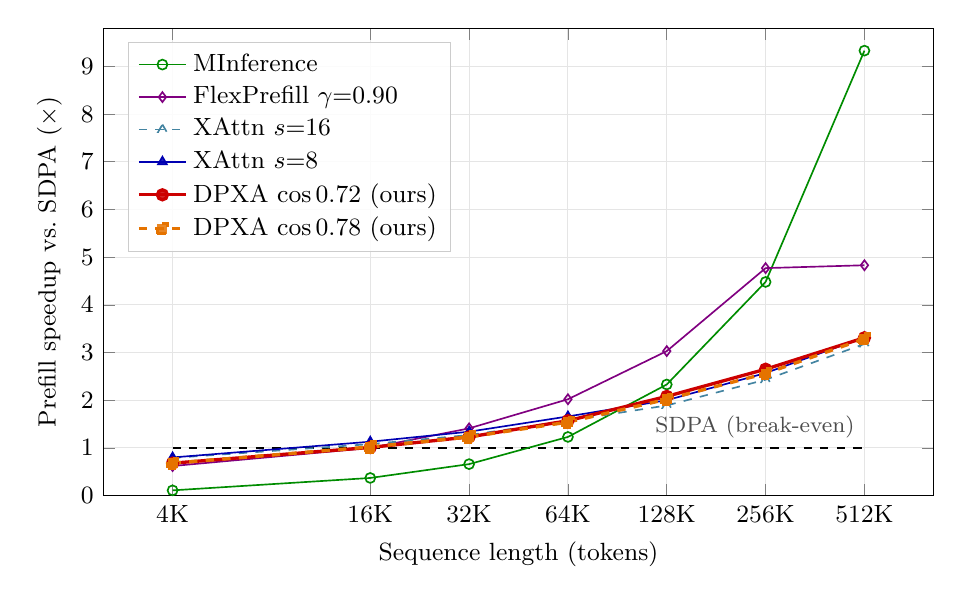
\begin{tikzpicture}
\begin{axis}[
    width=\linewidth, height=0.62\linewidth,
    xmode=log, log basis x=2,
    xtick={4096,16384,32768,65536,131072,262144,524288},
    xticklabels={4K,16K,32K,64K,128K,256K,512K},
    xlabel={Sequence length (tokens)},
    ylabel={Prefill speedup vs.\ SDPA ($\times$)},
    ymin=0, ymax=9.8,
    ytick={0,1,2,3,4,5,6,7,8,9},
    grid=both, grid style={gray!20},
    legend pos=north west,
    legend cell align=left,
    legend style={font=\small, fill=white, fill opacity=0.85, text opacity=1, draw=gray!40},
    tick label style={font=\small},
    label style={font=\small},
    mark size=1.8pt,
]
% break-even reference (SDPA)
\addplot[black, dashed, thick, forget plot] coordinates {(4096,1)(524288,1)};
\node[anchor=south east, font=\footnotesize, gray!60!black] at (axis cs:524288,1) {SDPA (break-even)};

\addplot[color=green!55!black, semithick, mark=o]
    coordinates {(4096,0.11)(16384,0.37)(32768,0.66)(65536,1.23)(131072,2.33)(262144,4.48)(524288,9.33)};
\addlegendentry{MInference}
\addplot[color=violet, semithick, mark=diamond]
    coordinates {(4096,0.62)(16384,1.00)(32768,1.41)(65536,2.02)(131072,3.03)(262144,4.77)(524288,4.83)};
\addlegendentry{FlexPrefill $\gamma{=}0.90$}
\addplot[color=cyan!60!black, semithick, dashed, mark=triangle]
    coordinates {(4096,0.79)(16384,1.08)(32768,1.27)(65536,1.57)(131072,1.89)(262144,2.43)(524288,3.18)};
\addlegendentry{XAttn $s{=}16$}
\addplot[color=blue!70!black, semithick, mark=triangle*]
    coordinates {(4096,0.80)(16384,1.13)(32768,1.34)(65536,1.66)(131072,2.00)(262144,2.57)(524288,3.32)};
\addlegendentry{XAttn $s{=}8$}
\addplot[color=red!80!black, very thick, mark=*]
    coordinates {(4096,0.68)(16384,1.01)(32768,1.23)(65536,1.57)(131072,2.08)(262144,2.65)(524288,3.31)};
\addlegendentry{DPXA cos\,0.72 (ours)}
\addplot[color=orange!90!black, very thick, dashed, mark=square*]
    coordinates {(4096,0.68)(16384,1.02)(32768,1.23)(65536,1.54)(131072,2.02)(262144,2.56)(524288,3.29)};
\addlegendentry{DPXA cos\,0.78 (ours)}
\end{axis}
\end{tikzpicture}
\caption{End-to-end prefill speedup relative to SDPA across sequence lengths on LLaMA-3.1 8B Instruct (4$\times$H100, layer-sharded). Points above the dashed break-even line (1.0$\times$) are faster than full attention. All methods are slower than SDPA at short contexts and cross break-even between 16K and 32K tokens; speedup then grows with sequence length as attention dominates the forward pass. Sequence lengths beyond 128K are outside LLaMA-3.1's native context and are used for latency benchmarking only. Table~\ref{tab:delta_tile_speedup} details the 128K operating point.}
\label{fig:dpxa_speedup_trend}
\end{figure}

\subsubsection{Cosine threshold ablation}
\label{sec:results_cos_ablation}

The cosine threshold $\tau$ controls how aggressively DPXA packs the delta representation used for tile scoring: a lower $\tau$ keeps fewer rows, making the score cheaper but less accurate, while a higher $\tau$ keeps more rows for a more accurate but more expensive score. We sweep $\tau \in \{0.70, 0.72, 0.75, 0.78, 0.80\}$ at fixed recall $r{=}0.90$ and report speedup, RULER, and LongBench. Because this sweep repeats the evaluation across five configurations, we use the reduced RULER (30 samples, 9 tasks) and reduced LongBench (9 tasks) setup described in the experimental setup, rather than the full setup used for the main DPXA results above.

The sweep trades scoring cost against tile count, and the two roughly cancel out (Table~\ref{tab:cos_speedup}). Lower thresholds score faster (1.6\% of full tile cost, 1{,}447 ms at cos\,0.70) but need more tiles to reach 90\% attention mass, since the ranking is coarser (19.0\% of tiles, 3{,}094 ms of attention). Higher thresholds give a sharper ranking that hits the same recall with fewer tiles (13.3\% of tiles, 2{,}140 ms of attention at cos\,0.80) but cost more to score (8.7\%, 2{,}885 ms). Because scoring and attention move in opposite directions, the end-to-end speedup stays roughly flat: it peaks at cos\,0.72 (2.10$\times$), stays close at cos\,0.70 (2.08$\times$), and only drops off at the high end (2.03$\times$ at cos\,0.78, 1.97$\times$ at cos\,0.80).

RULER is essentially lossless across the whole sweep (Table~\ref{tab:cos_ruler}): every setting lands within 0.4 points of the others, and cos\,0.78 (91.80), cos\,0.70 (91.69), and cos\,0.80 (91.58) all match or beat full attention (91.52). We think this is because of how RULER is built: it inserts target passages into unrelated filler text, and each insertion causes a sharp change in the hidden states. Delta thresholding is designed to catch exactly this kind of change, so the retrieval-critical tokens survive even under aggressive packing, and RULER accuracy holds at every threshold.

LongBench is more sensitive to $\tau$ (Table~\ref{tab:cos_longbench}). Accuracy peaks at cos\,0.72 (39.21) and falls off at both ends, most sharply at cos\,0.80 (38.61). cos\,0.72 is the best overall choice: fastest and best on LongBench. cos\,0.78 is the accuracy-maximizing choice, holding the best RULER score (91.80) at a still-good 2.03$\times$. cos\,0.80 is worse on both axes: slowest and weakest on LongBench. The useful range is roughly cos\,0.72 to cos\,0.78, and we carry both forward as the two settings compared against the other methods.

\begin{table}[!ht]
\centering
\caption{Prefill speedup at 128K tokens for the DPXA cosine-threshold sweep on LLaMA-3.1 8B Instruct, all at recall $r{=}0.90$ using the tuned scoring kernel. Speedup is end-to-end prefill relative to SDPA. Attention density is the fraction of the dense attention computed; Score\% is the fraction of full tile cost spent on scoring; Score ms and Attn ms are the scoring and attention phase latencies.}
\label{tab:cos_speedup}
\begin{tabular}{lrrrrr}
\toprule
Method & Speedup & Density & Score\% & Score (ms) & Attn (ms) \\
\midrule
DPXA cos\,0.70 & 2.08$\times$ & 19.0\% & 1.6\% & 1{,}447 & 3{,}094 \\
DPXA cos\,0.72 & 2.10$\times$ & 17.6\% & 2.3\% & 1{,}611 & 2{,}853 \\
DPXA cos\,0.75 & 2.09$\times$ & 15.7\% & 3.8\% & 1{,}954 & 2{,}545 \\
DPXA cos\,0.78 & 2.03$\times$ & 14.2\% & 6.3\% & 2{,}445 & 2{,}284 \\
DPXA cos\,0.80 & 1.97$\times$ & 13.3\% & 8.7\% & 2{,}885 & 2{,}140 \\
\bottomrule
\end{tabular}
\end{table}

\begin{table}[!ht]
\centering
\caption{RULER accuracy (\%) for the DPXA cosine-threshold sweep on LLaMA-3.1 8B Instruct (30 samples, 9 tasks), all at recall $r{=}0.90$.}
\label{tab:cos_ruler}
\begin{tabular}{lrrrrrrr}
\toprule
Method & 4K & 8K & 16K & 32K & 64K & 128K & Avg \\
\midrule
Full attention & 99.31 & 97.21 & 96.59 & 93.76 & 88.23 & 74.00 & 91.52 \\
\midrule
DPXA cos\,0.70 & 99.35 & 97.91 & 96.99 & 93.89 & 87.85 & 74.17 & 91.69 \\
DPXA cos\,0.72 & 99.43 & 97.56 & 96.93 & 94.32 & 88.09 & 72.74 & 91.51 \\
DPXA cos\,0.75 & 99.38 & 97.30 & 96.90 & 94.06 & 87.94 & 72.94 & 91.42 \\
DPXA cos\,0.78 & 99.35 & 97.64 & 96.83 & 94.44 & 87.73 & 74.78 & 91.80 \\
DPXA cos\,0.80 & 99.51 & 96.90 & 97.81 & 93.51 & 87.59 & 74.17 & 91.58 \\
\bottomrule
\end{tabular}
\end{table}

\begin{table*}[!ht]
\centering
\small
\caption{LongBench scores on LLaMA-3.1 8B Instruct (100 samples per task) for the DPXA cosine-threshold sweep, all at recall $r{=}0.90$. Task abbreviations as in Table~\ref{tab:longbench}.}
\label{tab:cos_longbench}
\resizebox{\linewidth}{!}{%
\begin{tabular}{lrrrrrrrrr r}
\toprule
Method & NQA & Qas & MFQ & HotP & 2Wiki & Mus & GovR & QMS & MNews & Avg \\
\midrule
Full attention & 31.91 & 43.06 & 56.25 & 54.87 & 47.97 & 34.88 & 34.47 & 25.27 & 27.15 & 39.54 \\
\midrule
DPXA cos\,0.70 & 31.13 & 41.85 & 56.74 & 53.42 & 49.10 & 31.59 & 34.51 & 25.59 & 26.63 & 38.95 \\
DPXA cos\,0.72 & 31.62 & 42.86 & 57.04 & 53.29 & 47.88 & 32.87 & 34.67 & 25.66 & 26.97 & 39.21 \\
DPXA cos\,0.75 & 31.26 & 42.35 & 56.76 & 53.11 & 49.27 & 32.12 & 35.11 & 25.27 & 26.51 & 39.08 \\
DPXA cos\,0.78 & 31.81 & 43.60 & 57.19 & 54.51 & 45.27 & 32.72 & 35.26 & 25.35 & 26.67 & 39.15 \\
DPXA cos\,0.80 & 30.23 & 43.37 & 56.26 & 51.92 & 46.73 & 32.03 & 34.91 & 25.49 & 26.54 & 38.61 \\
\bottomrule
\end{tabular}%
}
\end{table*}

\subsubsection{Cross-Model Generalization: Qwen2.5-7B}
\label{sec:results_qwen}

The results above use LLaMA-3.1 8B Instruct throughout. To check whether DPXA's behavior is specific to that model, we repeat the full RULER, LongBench, and speedup evaluation on Qwen2.5-7B-Instruct-1M, using the same two operating points (cos\,0.72 and cos\,0.78 at $r{=}0.90$) and the same baselines.


\paragraph{RULER.}

Table~\ref{tab:delta_tile_scoring_qwen} reports RULER accuracy on Qwen. MInference (90.35) and both XAttention strides (90.25 at $s{=}16$, 90.23 at $s{=}8$) tie full attention (90.33); DPXA trails by 1.4--2.2 points (88.89 at cos\,0.78 and 88.12 at cos\,0.72). FlexPrefill collapses to 53.50.

\begin{table}[!ht]
\centering
\caption{RULER accuracy (\%) comparing delta-based tile scoring against baseline and block-sparse methods on Qwen2.5-7B-Instruct-1M (100 samples, 13 tasks). DPXA and FlexPrefill are both at recall/coverage target $0.90$ ($r{=}0.90$ and $\gamma{=}0.90$ respectively). Best score per column in \textbf{bold}.}
\label{tab:delta_tile_scoring_qwen}
\begin{tabular}{lrrrrrrr}
\toprule
Method & 4K & 8K & 16K & 32K & 64K & 128K & Avg \\
\midrule
Full attention              & 94.10 & 93.67 & 93.54 & \textbf{91.17} & 88.07 & \textbf{81.41} & 90.33 \\
MInference                  & \textbf{94.16} & \textbf{94.00} & \textbf{94.03} & 90.99 & 87.68 & 81.23 & \textbf{90.35} \\
FlexPrefill                  & 74.39 & 61.74 & 55.66 & 59.71 & 32.38 & 37.10 & 53.50 \\
\midrule
XAttn $s=16$                & 94.02 & 93.55 & 93.66 & 90.85 & \textbf{88.21} & 81.22 & 90.25 \\
XAttn $s=8$                 & 94.06 & 93.53 & 93.60 & 91.02 & 87.96 & 81.23 & 90.23 \\
\midrule
DPXA cos\,0.72 & 94.01 & 92.38 & 92.56 & 87.45 & 83.69 & 78.60 & 88.12 \\
DPXA cos\,0.78 & 94.02 & 93.54 & 92.59 & 89.38 & 84.54 & 79.26 & 88.89 \\
\bottomrule
\end{tabular}
\end{table}

DPXA's gap isn't confined to one context length: it opens up from 16K onward and widens to roughly 3.5--4.4 points at 64K (Table~\ref{tab:delta_tile_scoring_qwen}), before narrowing again at 128K. To find its source, we break the 128K result down into its 13 individual RULER tasks (Table~\ref{tab:ruler_pertask_qwen}).

DPXA ties or beats XAttention on 11 of the 13 tasks. The whole gap comes from two tasks: variable tracking (vt) and common word extraction (cwe). Both ask the model to aggregate information spread across many positions, rather than retrieve a single needle, and DPXA collapses on both (53.8 and 13.8 at cos\,0.72, well below full attention's 75.8 and 27.3). This is DPXA's failure mode: strong on retrieval, weak on aggregation.

\begin{table*}[!ht]
\centering
\small
\caption{RULER per-task accuracy (\%) at 128K on Qwen2.5-7B-Instruct-1M (100 samples). ns1--3 = niah\_single\_1--3, mk1--3 = niah\_multikey\_1--3, mv = niah\_multivalue, mq = niah\_multiquery, vt = variable tracking, cwe = common words extraction, fwe = frequent words extraction, qa1--2 = question answering 1--2. vt and cwe are the aggregation tasks discussed in the text.}
\label{tab:ruler_pertask_qwen}
\resizebox{\linewidth}{!}{%
\begin{tabular}{lrrrrrrrrrrrrr}
\toprule
Method & ns1 & ns2 & ns3 & mk1 & mk2 & mk3 & mv & mq & vt & cwe & fwe & qa1 & qa2 \\
\midrule
Full attention & 100 & 97 & 100 & 100 & 96 & 89 & 82.8 & 99.5 & 75.8 & 27.3 & 81.0 & 69 & 41 \\
MInference     & 100 & 100 & 100 & 99  & 95 & 92 & 83.5 & 99.3 & 76.0 & 24.7 & 78.0 & 69 & 39.5 \\
\midrule
XAttn $s{=}16$ & 100 & 98 & 100 & 100 & 94 & 82 & 82.8 & 99.3 & 75.0 & 30.5 & 80.3 & 72 & 42 \\
XAttn $s{=}8$  & 100 & 98 & 100 & 100 & 97 & 84 & 82.8 & 99.0 & 73.0 & 28.9 & 79.3 & 70 & 44 \\
\midrule
DPXA cos\,0.72 & 100 & 98 & 100 & 97  & 90 & 84 & 86.0 & 99.3 & 53.8 & 13.8 & 82.0 & 70 & 48 \\
DPXA cos\,0.78 & 100 & 98 & 100 & 98  & 94 & 83 & 83.0 & 99.3 & 52.6 & 18.2 & 81.3 & 70 & 53 \\
\bottomrule
\end{tabular}%
}
\end{table*}

The Llama picture partially hides the weakness. Table~\ref{tab:ruler_pertask_llama_agg} shows the same two tasks at 128K on Llama. On cwe, full attention itself only reaches 1.6, and every method, DPXA included, is stuck near the same floor (0.5--2.8); there is no real signal in this task on Llama. But vt is not a floor effect: full attention reaches a meaningful 57.4, and DPXA holds up well, while XAttention pushes further ahead (61.4--74.6). DPXA's vt score on Llama is in fact higher than its vt score on Qwen (57.6 versus 52.6--53.8), even though Qwen's full attention is far stronger on this task (75.8 versus 57.4). This suggests the aggregation weakness is exaggerated on Qwen.

\begin{table}[!ht]
\centering
\caption{RULER accuracy (\%) at 128K on the two aggregation tasks (variable tracking, common words extraction) on LLaMA-3.1 8B Instruct (100 samples). On cwe, full attention is already near the floor and every method sits close to it; on vt, full attention is meaningful and DPXA holds up.}
\label{tab:ruler_pertask_llama_agg}
\begin{tabular}{lrr}
\toprule
Method & vt & cwe \\
\midrule
Full attention & 57.4 & 1.6 \\
MInference     & 61.8 & 0.5 \\
\midrule
XAttn $s{=}16$ & 61.4 & 1.6 \\
XAttn $s{=}8$  & 74.6 & 2.8 \\
\midrule
DPXA cos\,0.72 & 53.4 & 1.8 \\
DPXA cos\,0.78 & 57.6 & 2.2 \\
\bottomrule
\end{tabular}
\end{table}

\paragraph{LongBench.}

Table~\ref{tab:longbench_qwen} shows LongBench scores on Qwen. DPXA ties full attention (46.76): 46.19 at cos\,0.72 and 46.20 at cos\,0.78, tracking both XAttention variants (46.46 at $s{=}8$, 46.66 at $s{=}16$).

The RULER aggregation weakness does not show up in the LongBench average. DPXA is in fact the strongest method on RepoBench-P, beating full attention and both XAttention variants by a wide margin (35.15 and 36.90 versus 32.92 for full attention, 31.97 and 31.70 for XAttention). It also stays near-lossless on passage retrieval (97--98 versus 100).

The two tasks where DPXA falls short of full attention are MuSiQue (29.22--29.88 versus 32.70) and 2WikiMultiHopQA (52.46--53.31 versus 55.45), both multi-hop tasks that require combining evidence spread across several passages. This lines up with the RULER aggregation failure mode, though with only two tasks affected we can't say for certain that multi-hop QA and RULER's aggregation tasks share the same underlying cause.

MInference fails to complete two tasks (QMSum, RepoBench-P) at 128K, so its 16-task average is not directly comparable and is marked with $\dagger$.

\begin{table*}[!ht]
\centering
\small
\caption{LongBench scores on Qwen2.5-7B-Instruct-1M (100 samples per task, 16 tasks). DPXA and FlexPrefill are both at recall/coverage target $0.90$ ($r{=}0.90$ and $\gamma{=}0.90$ respectively). Task abbreviations as in Table~\ref{tab:longbench}. Best score per column in \textbf{bold}. $\dagger$MInference failed on 2 of 16 tasks (QMSum, RepoBench-P); its reported average is over the 14 completed tasks and is not directly comparable to the other rows.}
\label{tab:longbench_qwen}
\resizebox{\linewidth}{!}{%
\begin{tabular}{lrrrrrrrrrrrrrrrrr}
\toprule
Method & NQA & Qas & MFQ & HotP & 2Wiki & Mus & GovR & QMS & MNews & TREC & TQA & SAM & PCnt & PassR & LCC & RepoB & Avg \\
\midrule
Full attention               & 29.26 & 45.12 & 51.49 & \textbf{58.34} & 55.45 & 32.70 & 35.22 & 23.99 & 25.69 & 71.00 & 83.31 & 45.24 & 10.00 & \textbf{100.00} & \textbf{48.40} & 32.92 & 46.76 \\
MInference$^\dagger$         & 29.38 & 45.36 & 51.85 & 56.77 & 54.65 & \textbf{33.47} & 35.20 & --    & 25.98 & 71.00 & 83.31 & 46.32 & 10.00 & 99.00 & 47.63 & --    & (44.4)$^\dagger$ \\
FlexPrefill                  & 24.68 & 39.46 & 50.63 & 48.72 & 50.58 & 21.06 & 33.61 & \textbf{24.67} & 25.42 & 70.00 & 78.64 & 46.11 & 2.00 & 59.00 & 45.18 & 33.61 & 40.84 \\
XAttn $s{=}16$               & 29.84 & 44.74 & 51.41 & 57.63 & \textbf{55.62} & 32.60 & 34.84 & 24.00 & \textbf{26.09} & 70.00 & 83.18 & 46.00 & \textbf{12.00} & \textbf{100.00} & 46.70 & 31.97 & 46.66 \\
XAttn $s{=}8$                & \textbf{30.26} & 45.77 & \textbf{52.31} & 58.16 & 53.78 & 31.62 & 35.18 & 24.09 & 26.00 & 71.00 & 83.51 & 45.83 & 9.00 & \textbf{100.00} & 45.14 & 31.70 & 46.46 \\
\midrule
DPXA cos\,0.72 & 29.89 & \textbf{46.48} & 52.04 & \textbf{58.56} & 53.31 & 29.22 & 35.12 & 24.19 & 25.86 & 72.00 & 83.17 & \textbf{46.51} & 4.00 & 98.00 & 45.57 & 35.15 & 46.19 \\
DPXA cos\,0.78 & 28.16 & 42.79 & 50.85 & 55.59 & 52.46 & 29.88 & 35.11 & 24.33 & 25.57 & \textbf{74.00} & \textbf{83.84} & 46.18 & 10.00 & 97.00 & 46.52 & \textbf{36.90} & 46.20 \\
\bottomrule
\end{tabular}%
}
\end{table*}

\paragraph{Speedup.}

Figure~\ref{fig:dpxa_speedup_trend_qwen} traces end-to-end speedup on Qwen from 4K to 512K. XAttention and DPXA are reported only to 256K: both OOM at 512K on the block-sparse attention transients of the 4-GPU node, while SDPA, MInference, and FlexPrefill complete.

The overall picture matches Llama (Figure~\ref{fig:dpxa_speedup_trend}). MInference is the slowest method up to 64K and only catches up at 128K; it doesn't pass FlexPrefill until 512K, where it reaches 4.81$\times$, a smaller jump than the 9.33$\times$ it reaches on Llama. FlexPrefill leads from 4K to 256K, drops back (4.13$\times$ to 3.87$\times$) on 512K.

DPXA and XAttention track each other closely, but DPXA is clearly faster at 128K and 256K, reaching 1.57$\times$ and 1.81$\times$ versus 1.45$\times$ and 1.74$\times$ for XAttn $s{=}16$.

\begin{figure}[!ht]
\centering
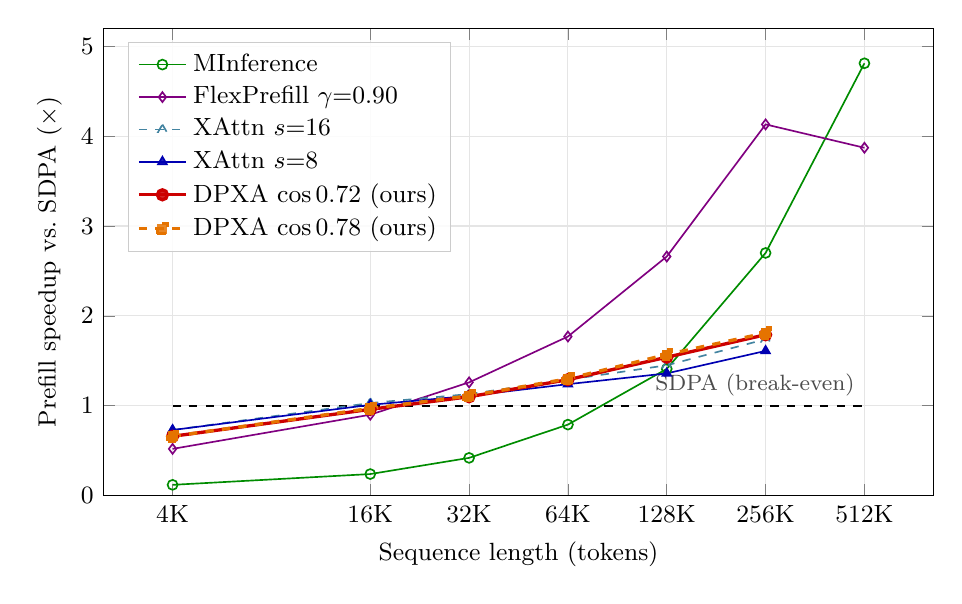
\begin{tikzpicture}
\begin{axis}[
    width=\linewidth, height=0.62\linewidth,
    xmode=log, log basis x=2,
    xtick={4096,16384,32768,65536,131072,262144,524288},
    xticklabels={4K,16K,32K,64K,128K,256K,512K},
    xlabel={Sequence length (tokens)},
    ylabel={Prefill speedup vs.\ SDPA ($\times$)},
    ymin=0, ymax=5.2,
    ytick={0,1,2,3,4,5},
    grid=both, grid style={gray!20},
    legend pos=north west,
    legend cell align=left,
    legend style={font=\small, fill=white, fill opacity=0.85, text opacity=1, draw=gray!40},
    tick label style={font=\small},
    label style={font=\small},
    mark size=1.8pt,
]
% break-even reference (SDPA)
\addplot[black, dashed, thick, forget plot] coordinates {(4096,1)(524288,1)};
\node[anchor=south east, font=\footnotesize, gray!60!black] at (axis cs:524288,1) {SDPA (break-even)};

\addplot[color=green!55!black, semithick, mark=o]
    coordinates {(4096,0.12)(16384,0.24)(32768,0.42)(65536,0.79)(131072,1.41)(262144,2.70)(524288,4.81)};
\addlegendentry{MInference}
\addplot[color=violet, semithick, mark=diamond]
    coordinates {(4096,0.52)(16384,0.90)(32768,1.26)(65536,1.77)(131072,2.66)(262144,4.13)(524288,3.87)};
\addlegendentry{FlexPrefill $\gamma{=}0.90$}
\addplot[color=cyan!60!black, semithick, dashed, mark=triangle]
    coordinates {(4096,0.73)(16384,1.03)(32768,1.13)(65536,1.29)(131072,1.45)(262144,1.74)};
\addlegendentry{XAttn $s{=}16$}
\addplot[color=blue!70!black, semithick, mark=triangle*]
    coordinates {(4096,0.73)(16384,1.01)(32768,1.11)(65536,1.24)(131072,1.36)(262144,1.61)};
\addlegendentry{XAttn $s{=}8$}
\addplot[color=red!80!black, very thick, mark=*]
    coordinates {(4096,0.66)(16384,0.96)(32768,1.10)(65536,1.29)(131072,1.54)(262144,1.79)};
\addlegendentry{DPXA cos\,0.72 (ours)}
\addplot[color=orange!90!black, very thick, dashed, mark=square*]
    coordinates {(4096,0.66)(16384,0.97)(32768,1.11)(65536,1.30)(131072,1.57)(262144,1.81)};
\addlegendentry{DPXA cos\,0.78 (ours)}
\end{axis}
\end{tikzpicture}
\caption{End-to-end prefill speedup relative to SDPA across sequence lengths on Qwen2.5-7B-Instruct-1M (4$\times$H100, layer-sharded). XAttention and DPXA are reported to 256K; both OOM at 512K on this hardware.}
\label{fig:dpxa_speedup_trend_qwen}
\end{figure}

\subsubsection{Video Understanding: Qwen2-VL}
\label{sec:results_video}

We test whether DPXA transfers beyond text to video understanding, using Qwen2-VL-7B-Instruct on Video-MME at 1 fps, the same video setup used in the XAttention paper. 

On video, packing by Euclidean distance works better than packing by cosine similarity, since it is also sensitive to magnitude rather than direction alone (see Ablations below). We therefore report DPXA with Euclidean packing at $\delta{=}15$, $r{=}0.90$ as the video operating point. We compare against full attention, XAttention at stride 16, MInference, and FlexPrefill, the same baselines used in the text experiments.

\paragraph{Benchmark.}

We measure two things on Video-MME: accuracy and speed. Accuracy is the rule-based score on the full test set (2,700 videos, 900 per duration bucket). Speedup is the attention-kernel latency relative to full attention, measured on a smaller timing sample of 10 videos per bucket. Unlike the text speedup tests, where we measure end-to-end latency, here we report attention latency only (scoring, block-selection, and packing, plus the actual block-sparse or dense attention kernel), since the end-to-end latency includes the whole vision decoding and dilutes the speedups. Both accuracy and speedup are broken down by video length: short (under 2 minutes), medium, and long (30 to 60 minutes). Table~\ref{tab:videomme_main} reports both.

DPXA at $\delta{=}15$ is our headline video result. It stays close to full attention (60.7 overall versus 62.1) and matches XAttention on quality, while being faster on long videos, the most crucial split. There DPXA scores 52.6 against XAttention's 51.7, and it runs at 1.33$\times$ full attention while XAttention only reaches 1.18$\times$.

The other DPXA settings trade accuracy for speed. $\delta{=}19$ overpacks and drops about 2 points overall (59.1), but on long videos it holds 51.1, close to XAttention (51.7), while reaching 1.79$\times$, the second highest long-video speedup after FlexPrefill. It is worth using only when speed is the priority.

MInference keeps the best accuracy of the sparse methods (62.4 overall) but is slower than full attention on every bucket (0.42$\times$ to 0.62$\times$). This matches our text speedup findings, where MInference only shows speedups past 128K. FlexPrefill is the fastest method (2.18$\times$ on long) and has solid overall accuracy retention, but it falls behind DPXA $\delta{=}15$ on long-video accuracy (51.6 versus 52.6).

\begin{table}[!ht]
\centering
\caption{Video-MME accuracy and prefill speedup on Qwen2-VL-7B-Instruct (Video-MME @ 1fps, no subtitles). Accuracy (\%) is on the full test set ($n{=}2700$). Speedup ($\times$full) is attention-kernel latency (\texttt{self\_attn\_ms}) relative to full attention on a 10-videos-per-bucket timing sample; higher is faster. DPXA rows use Euclidean packing with count-weighting off. Best accuracy per column in \textbf{bold}.}
\label{tab:videomme_main}
\begin{tabular}{lrrrrrr}
\toprule
 & \multicolumn{3}{c}{Accuracy (\%)} & \multicolumn{3}{c}{Speedup ($\times$full)} \\
\cmidrule(lr){2-4}\cmidrule(lr){5-7}
Method & Short & Med & Long & Short & Med & Long \\
\midrule
Full attention                    & 72.3 & 61.0 & 53.0 & 1.00 & 1.00 & 1.00 \\
MInference                        & \textbf{72.8} & 61.2 & \textbf{53.3} & 0.42 & 0.62 & 0.61 \\
FlexPrefill                        & 72.1 & \textbf{61.3} & 51.6 & 1.41 & 2.12 & 2.18 \\
XAttn $s{=}16$ ($r{=}0.90$)       & 72.0 & 59.9 & 51.7 & 0.95 & 1.22 & 1.18 \\
\midrule
DPXA $\delta{=}15$ ($r{=}0.90$)   & 71.1 & 58.6 & 52.6 & 0.98 & 1.21 & 1.33 \\
DPXA $\delta{=}19$ ($r{=}0.90$)   & 69.0 & 57.1 & 51.1 & 1.12 & 1.48 & 1.79 \\
\bottomrule
\end{tabular}
\end{table}

\paragraph{Ablations.}

We sweep cosine ($\tau \in \{0.72, 0.75, 0.80, 0.90\}$) and Euclidean ($\delta \in \{13, 15, 17, 19\}$) packing thresholds at matched recall $r{=}0.90$ on the Video-MME 200-video subset, with count-weighting off throughout (Table~\ref{tab:videomme_ablation_metric}). Euclidean is the stronger metric on long videos across the whole sweep, matching or beating XAttention's long score (44.6) at every threshold.

$\delta{=}15$ is the best operating point in the sweep: it has the highest overall score (60.5) and the strongest long score (50.0). Its scoring ratio (9.7\%) is higher than XAttention's (6.25\%), but it retains far fewer tiles (30.5\% versus 40.7\%), so the savings on the attention side outweigh the pricier scoring. We use $\delta{=}15$ as our operating point for the full-scale experiments.

$\delta{=}19$ trades accuracy for cost: overall drops to 57.5, but scoring ratio falls to 1.4\% and retained tiles to 23.6\%, both well below XAttention. This makes it a candidate fast operating point, though we have not yet confirmed it at full scale.




\begin{table}[!ht]
\centering
\caption{Packing metric ablation on Video-MME (200-video subset), Qwen2-VL-7B-Instruct, recall $r{=}0.90$, count-weighting off throughout.}
\label{tab:videomme_ablation_metric}
\begin{tabular}{llrrrrrr}
\toprule
Metric & $\tau$/$\delta$ & Overall & Short & Medium & Long & Retained tiles & Scoring ratio \\
\midrule
XAttn $s{=}16$ & -- & 59.0 & 75.0 & 59.7 & 44.6 & 40.7\% & 6.25\% \\
\midrule
Cosine & $\tau{=}0.90$ & 59.5 & 78.1 & 54.8 & 47.3 & 33.6\% & 45.8\% \\
Cosine & $\tau{=}0.80$ & 58.5 & 76.6 & 56.5 & 44.6 & 32.4\% & 14.2\% \\
Cosine & $\tau{=}0.75$ & 56.5 & 79.7 & 48.4 & 43.2 & 30.6\% & 7.4\% \\
Cosine & $\tau{=}0.72$ & 58.5 & 81.2 & 50.0 & 45.9 & 29.3\% & 5.0\% \\
\midrule
Euclidean & $\delta{=}13$ & 59.5 & 78.1 & 56.5 & 45.9 & 32.8\% & 21.2\% \\
Euclidean & $\delta{=}15$ & 60.5 & 76.6 & 56.5 & 50.0 & 30.5\% & 9.7\% \\
Euclidean & $\delta{=}17$ & 58.5 & 76.6 & 53.2 & 47.3 & 27.1\% & 3.8\% \\
Euclidean & $\delta{=}19$ & 57.5 & 75.0 & 48.4 & 50.0 & 23.6\% & 1.4\% \\
\bottomrule
\end{tabular}
\end{table}

% ==================== conclusion ====================
\section{Conclusion}

This thesis applied a single observation, that adjacent query and key vectors are highly similar, to three prefill acceleration methods: Delta-KV compression, DeltaXAttention, and delta-based tile scoring (DPXA). We summarize what each one showed.

\subsection{Delta-KV Compression}
Delta-KV compression halves the KV with cosine thresholding at 0.83 while retaining accuracy at a competitive level. The Triton kernels realize an end-to-end speedup, but the speedup is not dramatic. The theoretical maximum is 2x, and we cannot fully reach even that at the sequence lengths we tested. The method demonstrates the strengths of delta packing, but in this direct form the speedup is dominated by existing work. MInference reaches far higher speedups, up to 10x at one million tokens~\citep[Figure~1b]{jiang2024minference}, while the most Delta-KV compression can reach in this setup is 2x. This makes it impractical as a standalone method in this form.

\subsection{DeltaXAttention}
DeltaXAttention halves the KV operations of XAttention while trading some accuracy. However, XAttention can reach the same KV reductions natively, with a similar accuracy trade-off. XAttention translates these reductions directly into speedup because it skips entire blocks. DeltaXAttention does not realize speedups as easily: it does not reduce the number of tiles, which is what XAttention does natively, but instead reduces the number of KV loads and multiplications within each tile. In theory this can lower KV loading and multiplication time, but there is little motivation to build an implementation where these savings turn into real speedup.

\subsection{DPXA}

Among the baselines we tested, there is no silver bullet. Each method trades speed against accuracy and generalization in a different way.

The shape-oriented methods (MInference and FlexPrefill) excel in speedup, yet FlexPrefill struggles with model generalization and MInference realizes its speedup late.

MInference reaches exceptional speedups at very long contexts (256K to 512K), but it rises late and is slower than the baseline up to 128K. This shows up on video, where the longest clips sit around 32K tokens and MInference is much slower than full attention (0.42$\times$ to 0.62$\times$). It holds up accuracy and generalizes to models well. However, its RULER accuracy degrades at 128K on LLaMA (63.73 versus 74.46 for full attention). Overall, its solid performance proves its place in production.

FlexPrefill has a much smoother speedup curve. It delivers speedups at shorter contexts, reflected in its leading video speedups, even though it cannot reach the dramatic 512K speedup of MInference. Although it is competitive on speed, it suffers accuracy degradation on LLaMA RULER (87.45 versus 89.07) and especially on LongBench (44.78 versus 47.53), driven by the multi-hop tasks 2WikiMultiHopQA (38.53 versus 47.97) and MuSiQue (28.73 versus 34.88). More importantly, its accuracy breaks on every Qwen text benchmark (RULER 53.50 versus 90.33), which points to a cross-model generalization failure.

The block-sparse methods (XAttention and DPXA) retain accuracy better across the benchmarks, yet they cannot reach the impressive speedups of the shape-oriented methods.

XAttention generally has solid accuracy retention and cleanly generalizes to different models and modalities. On the Qwen RULER benchmark it scores considerably higher than DPXA (90.25 versus 88.12--88.89), but it falls back on LLaMA compared to DPXA (88.02 versus 89.02 on RULER). Its overall accuracy is tied with DPXA on video, yet on the long bucket DPXA has an advantage (52.6 versus 51.7).

DPXA shows that delta packing fits naturally as a tile importance estimator, and it gains a strong position in the training-free sparse attention arena.

It generally excels at accuracy retention and shows solid model and modality generalization. The one exception is the Qwen RULER aggregation tasks (variable tracking and common word extraction), where its accuracy degrades, though this does not carry over to the real-world LongBench benchmark.

It is the best method for accuracy retention on LLaMA and in long video understanding (excluding MInference on long video, since it runs about 2$\times$ slower than full attention there). Compared to XAttention, at all configurations and sequence lengths, it either matches or beats XAttention's speedup due to its much lighter scoring phase. The only reason we cannot say it dominates XAttention is the Qwen RULER aggregation degradation.

Overall, this thesis shows that adjacent token similarity is still largely unexplored in prefill acceleration. Delta-KV and DeltaXAttention demonstrate the potential but do not reach competitive results with the state of the art. DPXA applies the idea in a context where it naturally shines, and places itself in a competitive position among the state-of-the-art methods.






\subsection{Future Work}

Several directions could push DPXA further. The thresholding itself is the most immediate one. Q and K may benefit from separate thresholds, and later layers may tolerate more aggressive thresholding, since adjacent tokens are more similar there (Section~\ref{sec:observations}).

A second direction is to combine DPXA with the shape-oriented methods. On their block-sparse heads, FlexPrefill and MInference rank tiles by mean pooling, a fast but coarse importance estimator. DPXA's delta-based scoring could replace it as a sharper ranker while keeping their finer-grained sparsity and higher speedups.

A third direction is score normalization. Some tiles may score higher simply because they have more samples, rather than because they are more important. Count-weighting was designed to correct exactly this, but it hurt performance in our experiments, and we do not fully understand the theoretical mechanism behind that. A better normalization scheme for the tile scores, and a proper account of why the un-weighted score works so well, are left to future work.



\subsection{Strengths \& Limitations}

\paragraph{Strengths.}
Every method is run from its own codebase with its default configuration, so the comparison is fair to all of them. The baselines cover most of the strong work in the plug-and-play sparse attention domain, which places DPXA clearly against the current state of the art. All speedups are measured end-to-end rather than on isolated kernels, so no method benefits from a cherry-picked metric.

\paragraph{Limitations.}
There are a few things we did not cover. We did not test on InfiniteBench, which would add another long-context benchmark to the evaluation. We also skipped the longer RULER buckets (256K and 512K) because they are too expensive to run, though skipping these lengths is common in related work. Our Video-MME evaluation only uses the no-subtitles setting, so subtitled video understanding is left untested. Finally, we only evaluated understanding tasks, so video and image generation are left untested.

\newpage
\bibliographystyle{plainnat}
\bibliography{references}

\end{document}
